%%% LaTeX-Vorlage Version 1.8 %%%

% Grundlegende Dokumenteneigenschaften gemäß DHBW-Vorgaben
\documentclass[a4paper,fontsize=11pt,oneside,parskip=half,headings=normal,listof=nochaptergap]{scrreprt} 
% \usepackage{showframe} % nur für Kontrolle der Ränder 

%%% Präambel einbinden (mit Festlegungen gemäß DHBW-Vorgaben) %%%
%%% Präambel %%%
% hier sollten keine Änderungen erforderlich sein
%
\usepackage[utf8]{inputenc}   % Zeichencodierung UTF-8 für Eingabe-Dateien
\usepackage[T1]{fontenc}      % Darstellung von Umlauten im PDF

\usepackage{listings}         % für Einbindung von Code-Listings
\usepackage{xcolor}
\usepackage{booktabs}

\renewcommand\lstlistlistingname{Listingsverzeichnis}

\definecolor{codegreen}{rgb}{0,0.6,0}
\definecolor{codegray}{rgb}{0.5,0.5,0.5}
\definecolor{codepurple}{rgb}{0.58,0,0.82}
\definecolor{backcolour}{rgb}{0.95,0.95,0.92}

\lstdefinestyle{mystyle}{
  backgroundcolor=\color{backcolour},
  commentstyle=\color{codegreen},
  keywordstyle=\color{magenta},
  numberstyle=\tiny\color{codegray},
  stringstyle=\color{codepurple},
  basicstyle=\ttfamily\footnotesize,
  breakatwhitespace=false,
  breaklines=true,
  captionpos=b,
  keepspaces=true,
  numbers=left,
  numbersep=5pt,
  showspaces=false,
  showstringspaces=false,
  showtabs=false,
  tabsize=2,
  numberbychapter=false
}

\lstset{style=mystyle}

\lstset{literate=             % erlaubt Sonderzeichen in Code-Listings 
  {Ö}{{\"O}}1
{Ä}{{\"A}}1
{Ü}{{\"U}}1
{ß}{{\ss}}2
{ü}{{\"u}}1
{ä}{{\"a}}1
{ö}{{\"o}}1
{€}{{\euro}}1
}

\usepackage[
  inner=35mm,outer=15mm,top=25mm,
  bottom=20mm,foot=12mm,includefoot
]{geometry}                 % Einstellungen für Ränder
\usepackage{tabularx}
\usepackage[ngerman]{babel} % Spracheinstellungen Deutsch
\usepackage[babel,german=quotes]{csquotes} % deutsche Anf.zeichen
\usepackage{enumerate}      % anpassbare Nummerier./Aufz.
\usepackage{graphicx}       % Einbinden von Grafiken
\usepackage[onehalfspacing]{setspace} % anderthalbzeilig

\usepackage{blindtext}      % Textgenerierung für Testzwecke
\usepackage{color}          % Verwendung von Farbe 
\usepackage{pgfplots}      % für Diagramme
\pgfplotsset{compat=1.16}
\usepackage{tikz}
\usepackage{graphicx}
\usepackage{listings}
\usepackage{xcolor}
\definecolor{delim}{RGB}{20,105,176}
\definecolor{numb}{RGB}{106, 109, 32}
\definecolor{string}{rgb}{0.64,0.08,0.08}
\definecolor{backcolour}{rgb}{1,1,1}

\lstdefinelanguage{json}{
    basicstyle=\ttfamily\small\color{black},
    backgroundcolor=\color{backcolour},
    numbers=left,
    numberstyle=\small\color{gray},
    stepnumber=1,
    numbersep=8pt,
    showstringspaces=false,
    breaklines=true,
    frame=single,
    literate=
     *{0}{{{\color{numb}0}}}{1}
      {1}{{{\color{numb}1}}}{1}
      {2}{{{\color{numb}2}}}{1}
      {3}{{{\color{numb}3}}}{1}
      {4}{{{\color{numb}4}}}{1}
      {5}{{{\color{numb}5}}}{1}
      {6}{{{\color{numb}6}}}{1}
      {7}{{{\color{numb}7}}}{1}
      {8}{{{\color{numb}8}}}{1}
      {9}{{{\color{numb}9}}}{1}
      {\{}{{{\color{delim}{\{}}}}{1}
      {\}}{{{\color{delim}{\}}}}}{1}
      {[}{{{\color{delim}{[}}}}{1}
      {]}{{{\color{delim}{]}}}}{1}
      {,}{{{\color{delim}{,}}}}{1}
      {:}{{{\color{delim}{:}}}}{1},
    morestring=[b]",
    stringstyle=\color{red},   % Dies färbt alle Strings rot.
}
\usepackage[printonlyused]{acronym}        % für ein Abkürzungsverzeichnis

\usepackage[                % Biblatex
  backend=biber,
  bibstyle=_dhbw_authoryear,maxbibnames=99,
  citestyle=authoryear,
  uniquename=true, useprefix=true,
  bibencoding=utf8]{biblatex}
%kein Punkt am Ende bei \footcite
%http://www.golatex.de/footcite-ohne-punkt-am-schluss-t4865.html
\renewcommand{\bibfootnotewrapper}[1]{\bibsentence#1}


%Reihenfolge der Autorennamen
%   
% http://golatex.de/viewtopic,p,80448.html#80448
% Argumente: siehe http://texwelt.de/blog/modifizieren-eines-biblatex-stils/
\DeclareNameFormat{sortname}{% Bibliographie
  \ifnum\value{uniquename}=0 % Normalfall
  \ifuseprefix%
    {%
    \usebibmacro{name:family-given}
    {\namepartfamily}
    {\namepartgiveni}
    {\namepartprefix}
    {\namepartsuffixi}%
    }
    {%
    \usebibmacro{name:family-given}
    {\namepartfamily}
    {\namepartgiveni}
    {\namepartprefixi}
    {\namepartsuffixi}%
    }%
  \fi
  \ifnum\value{uniquename}=1% falls nicht eindeutig, abgek. Vorname 
    {%
    \usebibmacro{name:family-given}
    {\namepartfamily}
    {\namepartgiveni}
    {\namepartprefix}
    {\namepartsuffix}%
    }%
  \fi
  \ifnum\value{uniquename}=2% falls nicht eindeutig, ganzer Vorname 
    {%
    \usebibmacro{name:family-given}
    {\namepartfamily}
    {\namepartgiven}
    {\namepartprefix}
    {\namepartsuffix}%
    }%
  \fi
  \usebibmacro{name:andothers}}

\DeclareNameFormat{labelname}{% für Zitate
  \ifnum\value{uniquename}=0 % Normalfall
  \ifuseprefix%
    {%
    \usebibmacro{name:family-given}
    {\namepartfamily}
    {\empty}
    {\namepartprefix}
    {\namepartsuffixi}%
    }
    {%
    \usebibmacro{name:family-given}
    {\namepartfamily}
    {\empty}
    {\namepartprefixi}
    {\namepartsuffixi}%
    }%
  \fi
  \ifnum\value{uniquename}=1% falls nicht eindeutig, abgek. Vorname 
    {%
    \usebibmacro{name:family-given}
    {\namepartfamily}
    {\namepartgiveni}
    {\namepartprefix}
    {\namepartsuffix}%
    }%
  \fi
  \ifnum\value{uniquename}=2% falls nicht eindeutig, ganzer Vorname 
    {%
    \usebibmacro{name:family-given}
    {\namepartfamily}
    {\namepartgiven}
    {\namepartprefix}
    {\namepartsuffix}%
    }%
  \fi
  \usebibmacro{name:andothers}}


\DeclareFieldFormat{extrayear}{% = the 'a' in 'Jones 1995a'
  \iffieldnums{labelyear}
  {\mknumalph{#1}}
  {\mknumalph{#1}}}

\renewcommand*{\multinamedelim}{\addslash}
\renewcommand*{\finalnamedelim}{\addslash}
\renewcommand*{\multilistdelim}{\addslash}
\renewcommand*{\finallistdelim}{\addslash}

\renewcommand{\nameyeardelim}{~}

% Literaturverzeichnis: Doppelpunkt zwischen Name (Jahr): Rest 
% http://de.comp.text.tex.narkive.com/Tn1HUIXB/biblatex-authoryear-und-doppelpunkt
\renewcommand{\labelnamepunct}{\addcolon\addspace}

% damit die Darstellung für Vollzitate von Primärquellen in 
% Fußnoten später auf "nicht fett" geändert werden kann 
% (nur für Zitate von Sekundärliteratur relevant)
\newcommand{\textfett}[1]{\textbf{#1}}

% für Zitate von Sekundärliteratur:
\newcommand{\footcitePrimaerSekundaer}[4]{%
  \renewcommand{\textfett}[1]{##1}%
  \footnote{\fullcite[#2]{#1}, zitiert nach \cite[#4]{#3}}%  
  \renewcommand{\textfett}[1]{\textbf{##1}}%
}

% Im Literaturverzeichnis: Autor (Jahr) fett
\renewbibmacro*{author}{%
  \ifboolexpr{%
    test \ifuseauthor%
    and
    not test {\ifnameundef{author}}
  }
  {\usebibmacro{bbx:dashcheck}
    {\bibnamedash}
    {\usebibmacro{bbx:savehash}%
      \textfett{\printnames{author}}%
      \iffieldundef{authortype}
      {\setunit{\addspace}}
      {\setunit{\addcomma\space}}}%
    \iffieldundef{authortype}
    {}
    {\usebibmacro{authorstrg}%
      \setunit{\addspace}}}%
  {\global\undef\bbx@lasthash
    \usebibmacro{labeltitle}%
    \setunit*{\addspace}}%
  \textfett{\usebibmacro{date+extrayear}}}

% Sonderfall: Quelle ohne Autor, aber mit Herausgeber
% Name des Herausgebers wird fett gedruckt
\renewbibmacro*{bbx:editor}[1]{%
  \ifboolexpr{%
    test \ifuseeditor%
    and
    not test {\ifnameundef{editor}}
  }
  {\usebibmacro{bbx:dashcheck}
    {\bibnamedash}
    {\textfett{\printnames{editor}}%
      \setunit{\addcomma\space}%
      \usebibmacro{bbx:savehash}}%
    \usebibmacro{#1}%
    \clearname{editor}%
    \setunit{\addspace}}%
  {\global\undef\bbx@lasthash
    \usebibmacro{labeltitle}%
    \setunit*{\addspace}}%
  \textfett{\usebibmacro{date+extrayear}}}

% Anpassungen für deutsche Sprache
\DefineBibliographyStrings{ngerman}{%
  nodate = {{o.J.}},
  urlseen = {{Abruf:}},
  ibidem = {{ebenda}}
}

% keine Anführungszeichen beim Titel im Literaturverzeichnis
\DeclareFieldFormat[article,book,inbook,inproceedings,manual,misc,phdthesis,thesis,online,report]{title}{#1\isdot}

\newcommand{\literaturverzeichnis}{%
  % nur Literaturverzeichnis
  % (als eigenes Kapitel)
  \phantomsection
  \addcontentsline{toc}{chapter}{Literaturverzeichnis}
  \spezialkopfzeile{Literaturverzeichnis}
  \defbibheading{lit}{\chapter*{Literaturverzeichnis}}
  \label{chapter:quellen}
  \printbibliography[heading=lit,notkeyword=ausblenden]
} % mit DHBW-spezifischen Einstellungen

\usepackage[hidelinks]{hyperref}       % URL-Formatierung, klickbare Verweise

\usepackage{tocloft}        % für Verzeichnis der Anhänge


\newcounter{anhcnt}
\setcounter{anhcnt}{0}
\newlistof{anhang}{app}{}

\newcommand{\anhang}[1]{%
  \refstepcounter{anhcnt}
  \setcounter{anhteilcnt}{0}
  \section*{Anhang \theanhcnt: #1}
  \addcontentsline{app}{section}{\protect\numberline{Anhang \theanhcnt}#1}\par
}

\newcounter{anhteilcnt}
\setcounter{anhteilcnt}{0}

\newcommand{\anhangteil}[1]{%
  \refstepcounter{anhteilcnt}
  \subsection*{Anhang~\arabic{anhcnt}/\arabic{anhteilcnt}: #1}
  \addcontentsline{app}{subsection}{\protect\numberline{Anhang \theanhcnt/\arabic{anhteilcnt}}#1}\par
}

\renewcommand{\theanhteilcnt}{Anhang \theanhcnt/\arabic{anhteilcnt}}

% vgl. S. 4 Paket-Beschreibung tocloft 	
% Einrückungen für Anhangverzeichnis
\makeatletter
\newcommand{\abstaendeanhangverzeichnis}{
  \renewcommand*{\l@section}{\@dottedtocline{1}{0em}{5.5em}}
  \renewcommand*{\l@subsection}{\@dottedtocline{2}{2.3em}{6.5em}}
}
\makeatother

% Abbildungs- und Tabellenverzeichnis
% Bezeichnungen
\renewcaptionname{ngerman}{\figurename}{Abb.}
\renewcaptionname{ngerman}{\tablename}{Tab.}
% Einrückungen
\makeatletter
\renewcommand*{\l@figure}{\@dottedtocline{1}{0em}{2.3em}}
\renewcommand*{\l@table}{\@dottedtocline{1}{0em}{2.3em}}
\makeatother


\usepackage{chngcntr}                % fortlaufende Zähler für Fußnoten, Abbildungen und Tabellen
\counterwithout{figure}{chapter}
\counterwithout{table}{chapter}
\counterwithout{footnote}{chapter}

\usepackage[automark]{scrlayer-scrpage}
%% Definitionen für Kopf- und Fußzeile auf normalen Seiten
\defpagestyle{kopfzeile}
{% Kopfdefinition
  (\textwidth,0pt)    % Länge der oberen Linie,Dicke der oberen Linie       
  {} % Definition für linke Seiten im doppelseitigen Layout
    {} % Definition für rechte Seiten im doppelseitigen Layout      
    {  % Definition für Seiten im einseitigen Layout
      \makebox[0pt][l]{\rightmark}% 
      \makebox[\linewidth]{}% 
    }
  (\textwidth, 0.4pt) % Untere Linienlänge, Untere Liniendicke
}
{% Fußdefinition
  (\textwidth,0pt)    % Obere Linienlänge, Obere Liniendicke
  {} % Definition für linke Seiten im doppelseitigen Layout
    {} % Definition für rechte Seiten im doppelseitigen Layout
    {  % Definition für Seiten im einseitigen Layout
      \makebox[\linewidth]{}%
      \makebox[0pt][r]{\pagemark}%
    }
  (\textwidth, 0pt)   % Länge der unteren Linie,Dicke der unteren Linie
}

%% Definitionen für Kopf- und Fußzeile auf ersten Seiten eines Kapitels
\defpagestyle{kapitelkopfzeile}
{% Kopfdefinition
  (\textwidth,0pt)    % Länge der oberen Linie,Dicke der oberen Linie       
  {} % Definition für linke Seiten im doppelseitigen Layout
    {} % Definition für rechte Seiten im doppelseitigen Layout      
    {}  % Definition für Seiten im einseitigen Layout
  (\textwidth, 0pt) % Untere Linienlänge, Untere Liniendicke
}
{% Fußdefinition
  (\textwidth,0pt)    % Obere Linienlänge, Obere Liniendicke
  {} % Definition für linke Seiten im doppelseitigen Layout
    {} % Definition für rechte Seiten im doppelseitigen Layout
    {  % Definition für Seiten im einseitigen Layout
      \makebox[\linewidth]{}%
      \makebox[0pt][r]{\pagemark}%
    }
  (\textwidth, 0pt)   % Länge der unteren Linie,Dicke der unteren Linie
}

%% Definitionen für Kopf- und Fußzeile im Anhang und bei Quellenverzeichnisse
\newcommand{\spezialkopfzeileBezeichnung}{}
\defpagestyle{spezialkopfzeile}
{% Kopfdefinition
  (\textwidth,0pt)    % Länge der oberen Linie,Dicke der oberen Linie       
  {} % Definition für linke Seiten im doppelseitigen Layout
    {} % Definition für rechte Seiten im doppelseitigen Layout      
    {  % Definition für Seiten im einseitigen Layout
      \makebox[0pt][l]{\spezialkopfzeileBezeichnung}% 
      \makebox[\linewidth]{}% 
    }
  (\textwidth, 0.4pt) % Untere Linienlänge, Untere Liniendicke
}
{% Fußdefinition
  (\textwidth,0pt)    % Obere Linienlänge, Obere Liniendicke
  {} % Definition für linke Seiten im doppelseitigen Layout
    {} % Definition für rechte Seiten im doppelseitigen Layout
    {  % Definition für Seiten im einseitigen Layout
      \makebox[\linewidth]{}%
      \makebox[0pt][r]{\pagemark}%
    }
  (\textwidth, 0pt)   % Länge der unteren Linie,Dicke der unteren Linie
}

\newcommand\spezialkopfzeile[1]{%
  \renewcommand\spezialkopfzeileBezeichnung{#1}
  \pagestyle{spezialkopfzeile}
}

% Standard-Pagestyle auswählen
\pagestyle{kopfzeile}

% keine Kopfzeile anzeigen auf Seiten, auf denen ein 
% Kapitel beginnt oder das Inhalts-/Abbildungs-/Tabellenverzeichnis steht 
\renewcommand{\chapterpagestyle}{kapitelkopfzeile}
\tocloftpagestyle{kapitelkopfzeile}

		 % für schöne Kopfzeilen 

\usepackage{textcomp}            % erlaubt EUR-Zeichen in Eingabedatei
\usepackage{eurosym}             % offizielles EUR-Symbol in Ausgabe
\renewcommand{\texteuro}{\euro}  % ACHTUNG: nach hyperref aufrufen!

\usepackage{scrhack}             % stellt Kompatibilität zw. KOMA-Script
% (scrreprt) und anderen Paketen her

% Anpassung der Abstände bei Kapitelüberschriften
% (betrifft auch Inhalts-, Abbildungs- und Tabellenverzeichnis)
\renewcommand*\chapterheadstartvskip{\vspace*{-\topskip}}
\newcommand{\myBeforeTitleSkip}{1mm}
\newcommand{\myAfterTitleSkip}{10mm}
\setlength\cftbeforetoctitleskip{\myBeforeTitleSkip}
\setlength\cftbeforeloftitleskip{\myBeforeTitleSkip}
\setlength\cftbeforelottitleskip{\myBeforeTitleSkip}

\setlength\cftaftertoctitleskip{\myAfterTitleSkip}
\setlength\cftafterloftitleskip{\myAfterTitleSkip}
\setlength\cftafterlottitleskip{\myAfterTitleSkip}
%%% Ende der Präambel %%%


%%% Name der eigenen Literatur-Datenbank (ggf. anpassen) %%%
\bibliography{includes/literatur.bib}

\begin{document}
%%% Deckblatt einbinden %%% 
% Anpassungen nötig (Name, Titel etc.)
% HIER EDITIEREN: 
% Typ der Arbeit (für Deckblatt und Metadaten)
% - bitte Zutreffendes auswählen
%\newcommand{\typMeinerArbeit}{1. Projektarbeit}
%\newcommand{\typMeinerArbeit}{2. Projektarbeit}
%\newcommand{\typMeinerArbeit}{Seminararbeit}
\newcommand{\typMeinerArbeit}{Bachelorarbeit}

% Thema der Arbeit (für ehrenwörtliche Erklärung, ohne Umbrüche)
% HIER EDITIEREN: 
\newcommand{\themaMeinerArbeit}{Document Understanding Transformers in der Dokumentenverarbeitung}

% Vorname, Name der Autorin/des Autors (für Titelseite und Metadaten)
% HIER EDITIEREN:
\newcommand{\meinName}{Marc Novak}

\thispagestyle{empty}

\begin{spacing}{1}
  \begin{center}
    ~\vspace{0mm}

    % HIER EDITIEREN: Titel der Arbeit
    {\sffamily
      \LARGE
      % \Large  % bei sehr langen Titeln ggf. etwas kleinere Schriftart wählen
      \textbf{Document Understanding Transformers in der Dokumentenverarbeitung}

      \bigskip
      \textbf{}
    }


    \vspace{15mm}

    % Typ wird automatisch eingefügt (oben festlegen)
    {\Large \typMeinerArbeit}

    \vspace{1cm}

    % HIER ggf. EDITIEREN
    vorgelegt am \today

    \vspace{15mm}

    Fakultät Wirtschaft
    \medskip

    Studiengang Wirtschaftsinformatik
    \medskip

    % HIER EDITIEREN: Kurs eintragen
    Kurs WI2021G

    \vspace{10mm}

    von

    \vspace{10mm}

    % Vorname und Name wird automatisch eingefügt (oben festlegen) 
    {\large\textsc{\meinName}}

    \vspace{10mm}
  \end{center}

  \vfill

  % HIER EDITIEREN: Name des Unternehmens, Name der Betreuerin/des Betreuers
  \begin{tabular}{ll}
    Betreuer in der Ausbildungsstätte:        & DHBW Stuttgart:                                                    \\
    \hspace{0.4\linewidth}                    &                                                                    \\
    ELO Digital Office GmbH & $\langle$ Titel, Vorname und Nachname $\rangle$                    \\
    Dr. Konstantin Hauch
                                              & $\langle$ der/des wissenschaftlichen Betreuerin/Prüferin $\rangle$ \\
    Teamleiter Team KI                                                     \\
    \\
    Unterschrift der Betreuerin/des Betreuers                                                                      \\
  \end{tabular}


  \vspace{1cm}
  %(etwas Platz für die Unterschrift der Betreuerin/des Betreuers aus der Ausbildungsstätte)
\end{spacing}

% falls ein Vertraulichkeitsvermerk erforderlich ist,
% die Kommentarzeichen in den nachfolgenden Zeilen entfernen:

%\begin{center}
%\small
%\textbf{Vertraulichkeitsvermerk}:
%Der Inhalt dieser Arbeit darf weder als Ganzes noch in Auszügen \\
%Personen außerhalb des Prüfungs- und Evaluationsverfahrens zugänglich gemacht werden, sofern keine anders lautende Genehmigung des Dualen Partners vorliegt. 
%\end{center}

% Meta-Daten für PDF-Datei basierend auf obigen Angaben
\hypersetup{pdftitle={\themaMeinerArbeit}}
\hypersetup{pdfauthor={\meinName}}
\hypersetup{pdfsubject={\typMeinerArbeit\ DHBW Stuttgart \the\year}}


%%% Umstellung der Seiten-Nummerierung auf i, ii, iii ... %%%
\pagenumbering{Roman}
\cleardoublepage

%%% Inhalts-, Abbildungs-, Tabellenverzeichnisse %%%
% sollen einzeilig gesetzt werden, um Platz zu sparen 
\begin{spacing}{1}
  \tableofcontents
  \clearpage
  \chapter*{Abkürzungsverzeichnis}
\addcontentsline{toc}{chapter}{Abkürzungsverzeichnis}

\begin{acronym}[DHBW]
  % Argument definiert die Breite der ersten Spalte anhand des längsten vorkommenden Eintrags
  \acro{CRM}{Customer Relationship Management}
  \acro{DHBW}{Duale Hochschule Baden-Württemberg}
  \acro{IEEE}{Institute of Electrical and Electronics Engineers}
  \acro{ITIL}{IT Infrastructure Library}
  \acro{RoI}{Return-On-Invest}
  \acro{UCS}{Universal Character Set}
  \acro{UTF-8}{8-Bit UCS Transformation Format}
\end{acronym}

\vspace{2em}


  \clearpage
  \thispagestyle{kapitelkopfzeile}
  \listoffigures
  \phantomsection
  \addcontentsline{toc}{chapter}{Abbildungsverzeichnis} % Abb.verz. ins Inh.verz. aufnehmen

  \clearpage
  \listoftables
  \phantomsection
  \addcontentsline{toc}{chapter}{Tabellenverzeichnis}   % Tab.verz. ins Inh.verz. aufnehmen
  \clearpage
  \lstlistoflistings
  \addcontentsline{toc}{chapter}{Listingsverzeichnis}   % Lst.verz. ins Inh.verz. aufnehmen
\end{spacing}

%%% Umstellung der Seiten-Nummerierung auf 1, 2, 3 ... %%%
\cleardoublepage
\pagenumbering{arabic}

%%% Ihr eigentlicher Inhalt %%%
% Empfehlung: strukturieren Sie Ihren Text in einzelnen Dateien 
% und binden Sie diese hier mit \input{includes/dateiname.tex} ein
\chapter{Einleitung}

In den vergrangenen Jahren hat \ac{KI} in Unternehmen zunehmend an Bedeutung gewonnen. Seit 2019 verzeichnet der KI-Software Markt einen hohes Wachstum. Es wird davon ausgegangen, dass dieses Wachstum bis 2025 mit über 26 \% pro Jahr anhalten wird. \footcites[Vgl.][]{howarth_57_2024} Die Anwendungsbereiche von KI-Systemen sind vielfältig und reichen von der Automatisierung von Prozessen, über die Analyse von großen Datenmengen bis hin zur Vorhersage von zukünftigen Ereignissen.

Einer der beliebtesten Anwendungsbereiche von KI-Systemen ist die Dokumentenverarbeitung. Eine Befragung von 1420 IT-Fachkräften ergab, dass 28 \% der zugehörigen Unternehmen KI-Systeme zur Dokumentenverarbeitung einsetzen (s. Abb. \ref{fig:ai_tech_distribution}). \footcites[Vgl.][]{rackspace_most_2023} Die Dokumentenverarbeitung umfasst die Extraktion von Informationen, die Klassifizierung und die automatisierte Verarbeitung von Dokumenten.\footcites[Vgl.][S.1]{esposito_intelligent_2005} Die Verarbeitung von Dokumenten ist in vielen Unternehmen ein zeitaufwändiger Prozess, der durch den Einsatz von KI-Systemen automatisiert und beschleunigt werden kann.\footcites[Vgl.][S.11]{dutt_now_2024}

\pgfplotsset{compat=1.17} % Use the version of pgfplots you have installed

\begin{figure}[htb]
    \centering
\begin{tikzpicture}
    \begin{axis}[
        xbar, % Horizontal bars
        xmin=0, xmax=60, % Set the minimum and maximum x-coordinates
        width=11cm, height=9cm, % Width and height of the plot
        enlarge y limits=0.1, % Add some space between bars
        xlabel={Share of respondents in \%}, % Label for the x-axis
        symbolic y coords={
            Speech recognition,
            Image recognition,
            Facial recognition,
            Sales and marketing analytics,
            Document processing,
            Intelligent search,
            Recommender systems,
            Natural language processing,
            Predictive maintenance,
            Customer engagement,
            Computer vision
        },
        ytick=data, % Use the data for y-ticks
        nodes near coords,
        nodes near coords align={anchor=west}, % Add the percentage labels near the bars% Align the labels horizontally
        point meta=explicit symbolic % The meta data is explicitly given as symbolic text
    ]
    \addplot [draw=blue,fill=blue!30 ] coordinates {
        (51,Computer vision)[51\%]
        (47,Customer engagement)[47\%]
        (43,Predictive maintenance)[43\%]
        (38,Natural language processing)[38\%]
        (34,Recommender systems)[34\%]
        (31,Intelligent search)[31\%]
        (28,Document processing)[28\%]
        (26,Sales and marketing analytics)[26\%]
        (23,Facial recognition)[23\%]
        (18,Image recognition)[18\%]
        (13,Speech recognition)[13\%]};
    \end{axis}
\end{tikzpicture}
\caption[Gängigste Verwendungszwecke von KI in Unternehmen]{Gängigsten Verwendungszwecke von KI in Unternehmen\footnotemark} % Caption for the figure
    \label{fig:ai_tech_distribution} % Label for referencing the figure
\end{figure}
\footnotetext{Entnommen aus: \cite{rackspace_most_2023}}

Die Verarbeitung von gescannten Dokumenten, insbesondere von Rechnungen ist ein integraler Bestandteil der Dokumentenverarbeitung. Der Einsatz von \ac{OCR} ermöglicht die Digitalisierung und elektronische Weiterverarbeitung dieser Dokumente. Jeoch ist die Zuordnung der erkannten Zeichenketten zu interpretierbaren Metadaten oft von manueller Nachbearbeitung oder von regulären Ausdrücken abhängig. Eine weitere Hürde, welche sich bei der Extraktion von Informationen aus Rechnungen zeigt, sind die sehr heterogenen Vorlagen und Layouts, welche in der Verarbeitung zu Ungenauigkeiten führen kann. Die OCR kann hier nicht mehr sicher die erkannten Werte den entsprechenden Labeln zuordnen.\footcites[Vgl.][S.1]{rahal_information_2018} Die DMS-Software \ac{ELO} von ELO verarbeitet Rechnungen zurzeit mittels OCR. Die Anwendung von Transformer-Modellen, im Bereich des \ac{VDU} ermöglicht eine direkte kontextbasierte Weiterverarbeitung der Rechnungen.\footcites[Vgl.][S.1]{kim_ocr-free_2021}

Diese Arbeit untersucht neue Transformer-Modelle im Bereich des VDU. Es wird analysiert, wie diese Modelle, die ihren Ursprng in der natürlichen Sprachverarbeitung haben, auf die Interpretation visueller (layoutbasierter) und textueller Elemente in Dokumenten angewandt werden können. Weiterhin wird ein OCR-freier \ac{Donut} untersucht, um die Limitierungen von OCR bezüglich Laufzeit und Fehleranfälligkeit zu überwinden.\footcites[Vgl.][S.1]{kim_ocr-free_2021} Diese Arbeit umfasst die Bereitstellung einer Pipeline, welche vom Modelltraining des Donuts bis zur Endanwendung im Unternehmen ELO Digital Office GmbH reicht. 
Das Ziel dieser Arbeit ist es, die Anwendbarkeit von Transformer-Modellen im Bereich des \ac{VDU} zu untersuchen und die Leistungsfähigkeit der Pipeline zu evaluieren um folgende Forschungsfrage zu beantworten:
\begin{center}
    \emph{Kann die Anwendung von Document Understanding Transformer Modellen die Effizienz und Genauigkeit der Rechnungsverarbeitung im Vergleich zu bestehenden OCR-basierten Modellen steigern?}
\end{center} 
Um diese Frage zu beantworten wird anhand eines Benchmarks (detaillierte Beschreibung des Aufbaus folgt in Kapitel 3) die Leistungsfähigkeit der Donut-basierten Pipeline mittels diverser Metriken bemessen und zur Leistungsfähigkeit von OCR-basierten Modellen verglichen. Daher ist die Arbeit folgedermaßen strukturiert: \\Zunächst werden in Kapitel 2 die Grundlagen der Dokumentenverarbeitung und der Transformer-Modelle erläutert. In Kapitel 3 werden die zu untersuchenden Modelle ausgewählt. Des weiteren werden der experimentelle Ansatz und der Aufbau der Testumgebung und Datensätze beschrieben. In Kapitel 4 wird die Entwicklung der Pipeline und die Implementierung des Donut dargestellt. Kapitel 5 präsentiert die Ergebnisse des Experiments. Kapitel 6 diskutiert die Ergebnisse und zieht Schlussfolgerungen. Eine Zusammenfassung und ein Ausblick auf zukünftige Arbeiten schließen die Arbeit in Kapitel 7 ab. Mit dieser Strukturierung als Ausgangspunkt, folgt nun die detaillierte Betrachtung der Grundlagen der Dokumentenverarbeitung und der Transformer-Modelle in Kapitel 2.

\chapter{Theoretischer Hintergrund}
Im folgenden Kapitel werden die theoretischen Grundlagen für diese Arbeit erläutert, um ein Verständnis für die verwendeten Begriffe und Technologien zu schaffen. Zunächst wird ein kurzer Überblick über die \ac{OCR} gegeben. Anschließend werden die Grundlagen der Transformer-Modelle erläutert. Des Weiteren werden die Details des \ac{Donut} genauer betrachtet, um ein Verständnis für die Funktionsweise des Modells im Vergleich zu herkömmlichen Methoden zu schaffen.

\section{Grundlagen der OCR}
Dieser Abschnitt betrachtet die grundlegende Funktionsweise und die Anwendungsbereiche von OCR-Systemen, da auch heute noch die meisten Modelle der Dokumentenverarbeitung auf eine OCR für den textuellen Input angewiesen sind (siehe dazu bspw. LayoutLM3\footcites[Vgl. dazu ausführlich][]{huang_layoutlmv3_2022}, ERNIE\footcites[Vgl. dazu ausführlich][]{peng_ernie-layout_2022}, FastStrucText\footcites[Vgl. dazu ausführlich][]{zhai_fast-structext_2023} etc.). Der Abschnitt bietet einen grundlegenden Überblick über das Thema. Auf ein tieferes Verständnis und eine detaillierte Betrachtung der Funktionsweise von OCR-Systemen wird in dieser Arbeit nicht eingegangen, da der Fokus auf der Anwendung von Transformer-Modellen im Bereich der Dokumentenverarbeitung liegt. Dennoch darf die Relevanz von OCR-Systemen nicht unterschätzt werden, da sie in vielen \ac{SOTA}-Modellen immer noch als Basis für die Textextraktion dienen. 

Häufig liegen Informationen in handschriftlicher oder gedruckter Form vor. Diese Informationen können durch Scans als Bilder in Computern gespeichert werden, jedoch ist die weiterverarbeitung der Informationen schwierig. Das System kann nicht ohne weiteres auf den Text in den erfassten Bildern zugreifen, bzw. diesen Lesen. Das Ziel von OCR ist es, Text aus Bildern zu extrahieren. OCR-Systeme sind in der Lage, Text aus gescannten Dokumenten, Fotos oder anderen Bildern zu extrahieren und in maschinenlesbaren Text umzuwandeln. In einem solchen Format können die Informationen weiterverarbeitet und analysiert werden. Somit ermöglicht es OCR einer Maschine, Texte automatisch zu erkennen.\footcites[Vgl.][S.244]{hamad_detailed_2016}

Für eine hohe Qualität und Genauigkeit der Zeichenerkennung erwarten OCR-Systeme eine hohe Qualität der Eingabebilder. Die Qualität der Eingabebilder ist ein entscheidender Punkt für die Genauigkeit der Zeichenerkennung. Einige Faktoren stellen Herausforderungen für die OCR dar, darunter die Szenenkomplexität, ungleiche Beleuchtungsbedingungen, Verzerrungen, Unschärfe und Abbau, Aspektverhältnisse, die Kippung, die Schriftart und mehrsprachige Umgebungen.\footcites[Vgl.][S.245]{hamad_detailed_2016} Die Herausforderungen erfordern fortgeschrittene Algorithmen und Techniken, einschließlich maschinellem Lernen und künstlicher Intelligenz, um die Erkennungsrate zu verbessern. Diese Herausforderungen versucht das Donut-Modell zu überwinden, indem es auf Transformer-Modellen basiert und somit die Limitierungen von OCR-Systemen umgeht.\footcites[Vgl.][S.1]{kim_ocr-free_2021} Um die Ergebnisse von OCR-Systemen zu verbessern werden in der Literatur verschiedene Ansätze vorgeschlagen. Nguyen et. al. schlagen die Verwendung von BERT vor. Als kontextbasiertes Sprachmodell kann BERT die Genauigkeit der OCR-Systeme verbessern, indem es die Kontextinformationen der Wörter berücksichtigt. Die Autoren zeigen, dass BERT die Genauigkeit der OCR-Systeme durch Fehlererkennung und Korrektur verbessern kann.\footcites[Vgl.][S.335 f.]{nguyen_neural_2020} BERT und seine Derivate werden noch heute in vielen \ac{SOTA}-Modellen für die Textextraktion verwendet.\footcites[Vgl. dazu ausführlich][S.4084 ff.]{huang_layoutlmv3_2022} \footcites[Vgl. dazu ausführlich][S.2 ff.]{garncarek_lambert_2020}

Die Funktionsweise von OCR-Systemen kann in sechs Phasen unterteilt werden. Diese Phasen umfassen die Vorverarbeitung, die Segmentierung, die Normalisierung, die Merkmalsextraktion, die Klassifikation und die Postverarbeitung. Das Ziel der Vorverarbeitung ist es, das Eingabebild zu verbessern und zu bereinigen. Die Segmentierung ist der Prozess, bei dem das Bild in einzelne Zeichen oder Wörter aufgeteilt und vom Hintergrund des Bildes getrennt wird. Sie stellt die kritische und maßgebliche Komponente eines OCR-Systems dar. Die Normalisierung ist der Prozess, bei dem die Segmentierungsergebnisse in eine standardisierte Form gebracht werden. In der Merkmalsextraktionsphase extrahiert das System relevante Merkmale von Objekten oder Alphabeten und wandelt diese zu Merkmalsvektoren um. In der Klassifikationsphase werden die Eingaben unterschiedlichen Klassen zugeordnet.\footcites[Vgl.][S.244]{hamad_detailed_2016} Beispielsweise wird in der Klassifikationsphase die Rechnungsnummer einer Klasse \emph{Invoice-Nr.} zugeordnet und das Datum der Klasse \emph{Date}. Es gibt diverse Werkzeuge, um die Klassifikation durchzuführen. Laut Dongre u.a. ist das \emph{Character Classification Problem} verwandt mit der heuristischen Logik, da Menschen Zeichen und Dokumente durch Erfahrung und Lernen erkennen können. Da Neuronale Netze ebenfalls von heuristischer Natur sind, sollten sie sich besonders gut für solche Probleme eignen. \footcites[Vgl.][S.11]{dongre_review_2010} Hier bleibt jedoch unbeachtet, dass die Eignung auch von der Qualität des Netzes selbst abhängt, welche wiederrum von der Qualität der Trainingsdaten abhängig ist.\footcites[Vgl.][S.851]{kavzoglu_increasing_2009} Daher eignet sich das Neuronale Netz als Klassifikator nur dann besonders gut, wenn die Trainingsdaten von hoher Qualität sind und das Netz in der Klassifikation eine hohe Genauigkeit aufweist. In der Postverarbeitung werden abschließend die Klassifikationsergebnisse weiterverarbeitet und korrigiert, um die Genauigkeit des erkannten Textes zu erhöhen.\footcites[Vgl.][S.246 f.]{hamad_detailed_2016} Hier wird das zuvor genannte BERT-Modell eingesetzt, um die Genauigkeit der OCR-Systeme zu verbessern.\footcites[Vgl.][S.335 f.]{nguyen_neural_2020}

Die Anwendungsbereiche der OCR sind vielfältig. Sie reichen von der Digitalisierung von Dokumenten in der Rechtsbranche über die Verarbeitung von Checks in Banken bis ins Gesundheitswesen. Der für diese Arbeit relevante Verwendungszweck ist die Verarbeitung von Rechnungen. OCR-Systeme werden in vielen Organisationen eingesetzt, um Rechnungen zu digitalisieren und diese so zu überwachen.\footcites[Vgl.][S.247 f.]{hamad_detailed_2016}

\section{Transformer-Modelle}
Im Folgenden soll ein Verständnis für die Transformer-Modelle geschaffen werden, welche wiederrum die Grundlage für Donut bilden. Dabei werden zunächst die Herkunft und Relevanz der Transformer-Modelle (folgend auch Transformer genannt) erläutert. Anschließend wird die Funktionsweise der Modelle genauer betrachtet. Dabei werden Schlüsselkonzepte wie die Aufmerksamkeit und das Positional Encoding, sowie die Architektur der Modelle erläutert. Seit der Einführung der Transformer in 2017 durch Vaswani et al. \footcites{vaswani_attention_2017} sind diese zum de facto Standard für eine Reihe verschiedener \ac{NLP} Aufgaben geworden. \ac{NLP} ist ein Teilbereich der Informatik, welcher es ermöglchen soll Computer Sprache auf eine \emph{natürliche} Art und Weise zu verstehen, so wie Menschen. Typischerweise refferenziert dies Aufgaben wie das Verstehen von Gefühlen in Texten, die Spracherkennung und das generieren von Antworten auf Fragen. \footcites[Vgl.][S.1]{beysolow_ii_applied_2018} Mittlerweile werden Transformer in den bekanntesten und meist genutzen Modellen der Welt verwendet, darunter BERT und GPT. \footcites[Vgl.][S. 1]{tunstall_natural_2022} Die beachtliche Leistungsfähigkeit der Transformer zeigt sich in den Benutzerzahlen von ChatGPT (ein ChatBot von OpenAI welcher auf den Transformer-Modellen basiert). Innerhalb von fünf Tage nach der Veröffentlichung des Modells hatte ChatGPT bereits eine Millionen Nutzer. Im Vergleich dazu brauchte Instagram zwei und halb Monate, um die gleiche Anzahl an Nutzern zu erreichen. \footcites[Vgl.][]{buchholz_infographic_2023} Den Status quo, vor der Entwicklung der Transformer, bildeten die \ac{RNN} und \ac{LSTM} Modelle. Transformer erzielen sowohl in der Leistungsfähigkeit als auch in den Trainingskosten bessere Ergebnisse als seine Vorgänger. \footcites[Vgl.][S. 1]{tunstall_natural_2022}

\subsection{Konzepte und Terminologie der Transformer-Modelle}
%TODO: Complete Chapter: Self-Attention, Multi-Head Attention, Positional Encoding, Encoder-Decoder Architektur

\subsection{Encoder-Decoder Architektur}
Das ursprüngliche Transformer-Modell, präsentiert von Vaswani et al. in 2017, basiert auf einer \emph{Encoder-Decoder} Architektur. Diese Architektur eignet sich besonder gut für Situationen, in welchen es sich sowohl bei der Ein- als auch der Ausgabe um Sequenzen handelt. Der Encoder wandelt die Eingabe von einer Sequenz in eine numerische Repräsentation um, welche häufig als \emph{last hidden state} bezeichnet wird. Dieser Zustand wird dann in den Decoder übergeben, welcher die Ausgabesequenz generiert. \footcites[Vgl.][S. 3]{tunstall_natural_2022}.

Der Aufbau der Encoder-Schicht kann Abb. \ref{fig:encoder-block} entnommen werden. Der Text wird zunächst in sog. \emph{Token Embeddings} umgewandelt. Das Ziel der Token Embeddings ist es Wörter, welche in Tokens umgewandelt wurden, in ihrem Kontext zu repräsentieren, da Wörter in verschiedenen Kontexten unterschiedliche Bedeutungen haben können. \footcites[Vgl.][S.692]{popa_towards_2021} %FIXME: Quelle selbst sagt Seite 2 aber das Magazin sagt 692...
Die Token Embeddings werden dann um \emph{Positional Embeddings} ergänzt. Diese repräsentieren die Position eines Tokens in einem Satz. Die Embeddings werden in den Encoder eingespeist, welcher die Eingabe in eine numerische Repräsentation umwandelt. Die Rolle des Encoders ist es die eingegangen Embeddings zu aktualisieren. Es sollen Repräsentationen von Tokens produziert werden, welche um kontextuelle Informationen angereichert sind. Beispielsweise wird das Wort \emph{Apple} aktualisiert, sodass es in einem unternehmerischen Kontext verstanden wird, wenn die Worte \emph{keynote} und \emph{phone} sich in der Nähe befinden. Konkret laufen die Embeddings durch zwei Schichten eines Encoder-Blocks: \footcites[Vgl.][S.58 ff.]{tunstall_natural_2022}
\begin{itemize}
    \item \emph{Multi-Head Attention Layer}
    \item \emph{Feed-Forward Layer}
\end{itemize}

\begin{figure}[h]
    \centering
    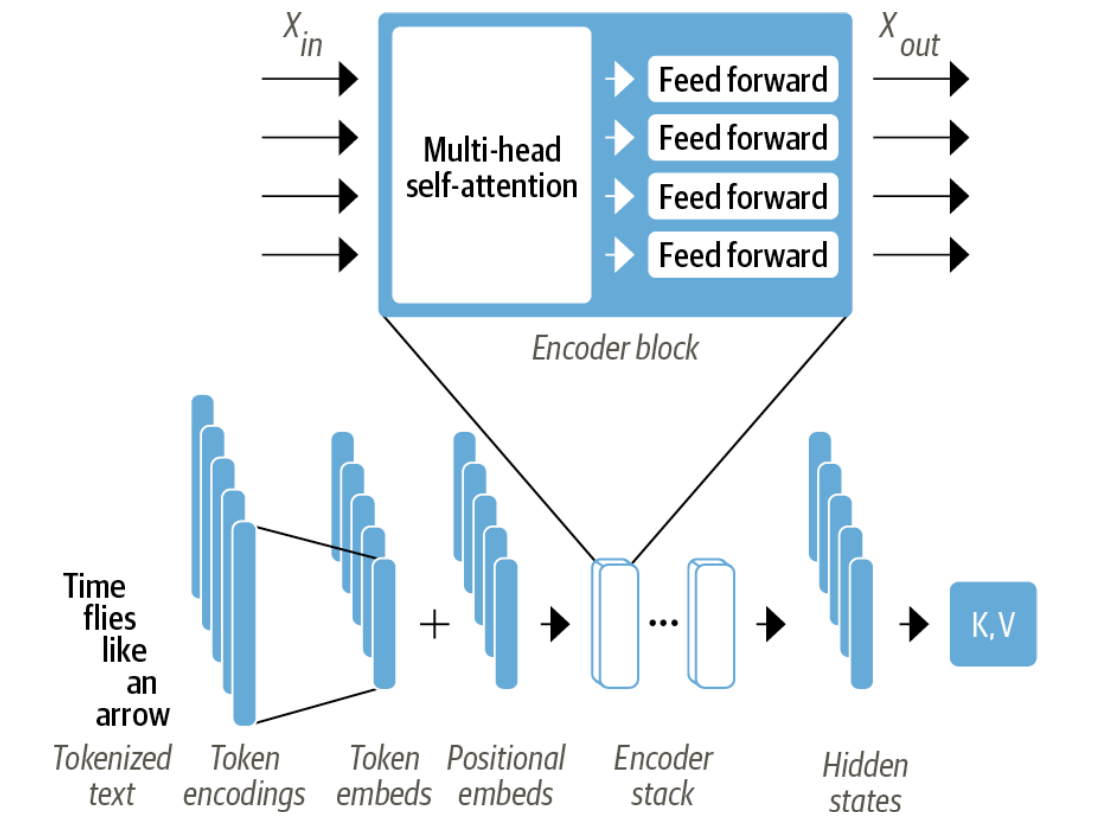
\includegraphics[height=80mm]{graphics/encoder-block.png}
    \caption[Aufbau eines Encoder-Blocks]{Aufbau eines Encoder-Blocks \footnotemark}
    \label{fig:encoder-block}
\end{figure}
\footnotetext{Entnommen aus: \cite{tunstall_natural_2022}, S.60}
%TODO: Complete Chapter: Decoder, Zusammenspiel, Bottleneck -> Relevanz Attention


\chapter{Methodik}
Das folgende Kapitel hat es zum Ziel, den experimentellen Ansatz und die Methodik dieser Arbeit zu beschreiben. Es soll deutlich werden, wie die Forschungsfrage beantwortet wird und welche Schritte dafür notwendig sind. Zunächst werden die zu untersuchenden Modelle aufgelistet. Folgend wird die Anwendung der Forschungsmethode und die entsprechenden Metriken erklärt. Anschließend werden der Aufbau der Testumgebung und die verwendeten Datensätze beschrieben. 
\section{Auswahl der zu untersuchenden Modelle}
Zunächst gilt es die zu untersuchenden Modelle auszuwählen. Die Auswahl der Modelle erfolgt auf Basis der Forschungsfrage und der Zielsetzung dieser Arbeit. Es sollen Modelle untersucht werden, die im Bereich des \ac{VDU} eingesetzt werden können. Die Modelle sollen in der Lage sein, visuelle und textuelle Elemente in Dokumenten zu interpretieren. 

\textbf{Donut:} Das zentrale Modell dieser Arbeit ist \ac{Donut}, gegen welches die OCR-basierten Modelle als Vergleichs- bzw. Referenzmodelle herangezogen werden. Diese Herangehensweise ermöglicht es, die Stärken, Schwächen und Besonderheiten von Donut im Vergleich zu alternativen Methoden des \ac{VDU} zu identifizieren. Es gibt zwar jüngere Nachfolger von \ac{Donut}, jedoch wird in dieser Arbeit ausschließlich Donut untersucht, da es das erste Modell seiner Art ist und die Grundlage für die nachfolgenden Modelle bildet. Es ist in dieser Hinsicht schon etablierter als bspw. \ac{DUBLIN}. Ferner gibt es bereits mehr Forschungsergebnisse zu \ac{Donut} als zu jüngeren Modellen und die Verfügbarkeit von Open-Source Implementierungen ist gegeben.

\textbf{BERT:} \ac{BERT} ist ein rein textbasiertes Modell, welches in der natürlichen Sprachverarbeitung eingesetzt wird. In der Literatur wird es im Bereich des \ac{VDU} einer OCR häufig nachgelagert, um Ergebnisse zu verbessern. \footcites[Vgl. dazu ausführlich][]{nguyen_neural_2020}[Vgl. dazu ausführlich][]{jiang_evaluating_2021} Noch heute wird \ac{BERT} in vielen Forschungen als Vergleichsmodell herangezogen. Eine Eigenschaft, die jedoch beachtet werden muss, ist, dass \ac{BERT} nicht in der Lage ist, visuelle Elemente zu interpretieren. Es handelt sich lediglich um einen Encoder-basierten Transformer, der um keine layoutbasierten Informationen angereichert wurde, \footcites[Vgl. dazu ausführlich][]{devlin_bert_2018} anders als bspw. LayoutLMv3. Es werden in dieser Arbeit die Ergebnisse von \ac{BERT} zu \ac{Donut} im Rahmen der Namend Entity Recognition und der Informationsextraktion verglichen.

%TODO: Fußnote für die Lizenzbedingung anpassen
\textbf{LayoutLMv3:} LayoutLMv3 ist ein performantes und etabliertes OCR-abhängiges Modell. LayoutLM wurde stetig optimiert, bis es Version 3 erreichte. Im FUNSD-Benchmark schneidet es deutlich besser ab als Donut und auch im CORD-Benchmark sind die Ergebnisse besser. \footcites[Vgl. dazu ausführlich][]{huang_layoutlmv3_2022} Der Source-Code von LayoutLMv3 ist zwar einsehbar, jedoch ist das Modell nicht Open-Source. LayoutLMv3 unterliegt strengen Lizenzbedingungen\footcites[Vgl.][]{noauthor_microsoftlayoutlmv3-base_2023} und darf nur für nicht-kommerzielle Zwecke wie Forschung verwendet werden. Daher impliziert der Vergleich von LayoutLMv3 zu Donut mehrere Punkte. Zum einen wird eine Implikation hinsichtlich der Gegenüberstellung von Open-Source und proprietären Modellen gezogen. Zum anderen wird untersucht, ob die proprietäre Implementierung von LayoutLMv3 einen Vorteil gegenüber Donut bringt. Nicht zuletzt wird untersucht, wie OCR-freie Modelle gegenüber OCR-abhängigen Modellen in einer heterogenen, produktionsähnlichen Landschaft an Daten abschneiden.

\section{Metriken des Experiments}
Zuzüglich zu den Modellen, die untersucht werden, ist es notwendig, die Leistungsfähigkeit der Modelle anhand von Metriken zu bewerten. Die Metriken sollen die Effizienz und Genauigkeit der Modelle messen. Sie sollen es ermöglichen, die Modelle miteinander zu vergleichen und die Forschungsfrage bzw. die noch folgenden Hypothesen zu beantworten. Die Metriken, die in dieser Arbeit verwendet werden, sind: Accuracy, F1-Score und \ac{GPUh}. In den folgenden Passagen werden die Metriken und ihre Bedeutung erläutert. Zunächst ist es wichtig, die grundlegende Terminologie zu erläutern, um anschließend die jeweiligen Metriken unter Zunahme der Terminologie erklären zu können. Die Bezeichnungen \emph{positive Klasse} und \emph{negative Klasse} beziehen sich auf die Klassen, wie sie in einer Konfusionsmatrix definiert sind. Die positive Klasse ist die Klasse, die identifiziert werden soll, die negative Klasse ist die Klasse, die nicht identifiziert werden soll. In dieser Arbeit beschreibt \ac{TP} eine Information, die extrahiert wurde und tatsächlich im Dokument vorhanden ist. Ein \ac{TN} liegt vor, wenn eine bestimmte Information oder Entität, wie beispielsweise die Rechnungsnummer, im Dokument nicht vorhanden ist und vom Modell auch nicht extrahiert wurde. Ein \ac{FP} tritt auf, wenn das Modell eine Information oder Entität fälschlicherweise extrahiert, die tatsächlich nicht im Dokument vorhanden ist, oder wenn es eine Information falsch zuordnet, wie zum Beispiel die Fehlinterpretation einer IBAN als Rechnungsnummer. Ein \ac{FN} beschreibt eine Situation, in der eine im Dokument vorhandene und relevante Information, wie die Rechnungsnummer, vom Modell nicht erkannt oder extrahiert wurde. Diese Kategorisierung hilft, die Genauigkeit der Entitätsextraktion zu bewerten, indem sie nicht nur das Vorhandensein, sondern auch die korrekte Identifikation und Zuordnung der Entitäten berücksichtigt.\footcites[Vgl.][]{pawan_confusion_2019}

\textbf{Accuracy:} Die Accuracy ist eine Standardmetrik, die den Anteil der korrekt identifizierten Fälle (sowohl positiv als auch negativ) im Verhältnis zur Gesamtzahl aller Fälle misst. Sie bietet einen schnellen Überblick über die Effektivität eines Modells. Allerdings kann sie in Situationen mit ungleichen Klassenverteilungen irreführend sein, da sie die Effektivität in den einzelnen Klassen nicht differenziert betrachtet. Zusammen mit allen weiteren Metriken befinden sich die Werte zwischen 0 und 1. Ein hoher Wert für die Accuracy zeigt an, dass ein großer Anteil der gesamten Vorhersagen des Modells korrekt ist, sowohl positive als auch negative Vorhersagen. Sie ist besonders aussagekräftig, wenn die Klassen im Datensatz ausgewogen sind.
Ein niedriger Wert für die Accuracy deutet darauf hin, dass das Modell viele Fehler macht, was auf Probleme mit der Modellierung, der Datenqualität oder einer Klassenimbalance hindeuten kann.\footcites[Vgl.][S. 508]{naser_error_2023}
\begin{equation}
    {Accuracy} = \frac{TP + TN}{TP + TN + FP + FN} 
\end{equation}


\textbf{F1-Score:} Der F1-Score ist ein harmonisches Mittel aus Präzision und Recall, das heißt, er berücksichtigt sowohl die Fähigkeit des Modells, relevante Informationen korrekt zu identifizieren (Präzision), als auch die Fähigkeit, alle relevanten Informationen zu erfassen (Recall). Ein niedriger F1-Score weist auf eine oder mehrere der folgenden Situationen hin: Das Modell kann relevante Informationen nicht korrekt identifizieren, es kann relevante Informationen nicht vollständig erfassen oder es kann irrelevante Informationen nicht ausschließen. In jedem Fall führt ein niedriger F1-Score zu einer geringeren Genauigkeit der Informationsgewinnung, was wiederum zu einer ineffizienten und ungenauen Dokumentenverarbeitung führt.

\begin{itemize}
    \item Precision (Präzision) misst den Anteil der korrekt identifizierten positiven Fälle im Verhältnis zu allen Fällen, die vom Modell als positiv eingestuft wurden. Eine hohe Precision bedeutet, dass ein hoher Anteil der positiven Vorhersagen des Modells tatsächlich korrekt ist, was bei Aufgaben wichtig ist, bei denen die Kosten für falsch positive Ergebnisse hoch sind.
    Eine niedrige Precision zeigt an, dass viele der als positiv klassifizierten Fälle falsch sind, was in Szenarien, in denen Vertrauen in das Ergebnis entscheidend ist, problematisch sein kann. \footcites[Vgl.][S. 508]{naser_error_2023}
    \begin{equation}
        Precision = \frac{TP}{TP + FP}
    \end{equation}
    \item Recall (Sensitivität) gibt den Anteil der korrekt identifizierten positiven Fälle im Verhältnis zu allen tatsächlich positiven Fällen an. Ein hoher Recall-Wert zeigt, dass das Modell einen großen Anteil der tatsächlich positiven Fälle korrekt erkennt und extrahiert. Dies ist wichtig in Situationen, wo das Übersehen von positiven Fällen schwerwiegende Folgen haben kann. Ein niedriger Recall bedeutet, dass das Modell viele tatsächliche positive Fälle nicht erkennt, was bei kritischen Anwendungen wie medizinischen Diagnosen oder Betrugserkennung zu ernsthaften Problemen führen kann. \footcites[Vgl.][S. 508]{naser_error_2023}
    \begin{equation}
        Recall = \frac{TP}{TP + FN}
    \end{equation}
\end{itemize}

Indem der F1-Score, Precision und Recall vereint, bietet er eine robuste Bewertung der Modellleistung, die sowohl die Vermeidung von Falsch-Positiven als auch die korrekte Identifikation aller positiven Fälle berücksichtigt. Ein hoher F1-Score ist ein Indikator dafür, dass das Modell sowohl eine hohe Precision als auch einen hohen Recall erreicht hat, was auf eine ausgewogene Leistung in Bezug auf die Vermeidung von falsch positiven und das Übersehen von tatsächlich positiven Fällen hindeutet.
Ein niedriger F1-Score zeigt, dass das Modell entweder viele relevante Fälle übersieht oder viele irrelevante Fälle fälschlicherweise als positiv einstuft, was auf eine schlechte Gesamtleistung des Modells hinweist.\footcites[Vgl.][S. 509]{naser_error_2023}
\begin{equation}
    F_{1} = 2 \cdot \frac{Precision \cdot Recall}{Precision + Recall}
\end{equation}

\textbf{GPUh:} \ac{GPUh} beziehen sich auf die Rechenzeit, die für das Feintuning auf GPU-Hardware benötigt wird. Diese Metrik ist besonders relevant, um die Kosten der Modellentwicklung und -anwendung zu bewerten. Sie ist von großer Bedeutung für kleinere Organisationen oder Einzelpersonen, die möglicherweise nicht über die Ressourcen verfügen, um umfangreiche Datensätze für das Training eigener Modelle zu sammeln oder teure GPU-Ressourcen über längere Zeiträume zu nutzen.

\section{Forschungsdesign}
\subsection{Voraussetzungen für das Experiment}
Das Forschungsdesign dieser Arbeit basiert auf einem experimentellen Ansatz, der darauf abzielt, die Performance von KI-Modellen speziell im Bereich der Informationsextraktion aus Dokumenten, zu untersuchen und zu vergleichen. Dabei liegt der Fokus auf der Evaluation des Donut-Modells im Vergleich zu OCR-abhängigen Modellen wie LayoutLMv3 und BERT, insbesondere unter Produktivbedingungen, die über die Rahmenbedingungen standardisierter Benchmark-Datensätze hinausgehen.

In einem Experiment müssen diverse Voraussetzungen erfüllt werden. Das Untersuchungsobjekt sind im Fall dieser Arbeit die zuvor genannten KI-Modelle und deren Performance in der Informationsextraktion aus Dokumenten. Der Beobachter ist der Forscher, der die Modelle trainiert und evaluiert, sowie die Monitoring-Tools, welche für die Beobachtung des Aufwands der Genauigkeit der Modelle zuständig sind. Der Versuchsaufbau gestaltet sich wie folgt: Zunächst werden die Modelle auf den gleichen Trainingsdatensatz trainiert (Finetuning) und anschließend auf einem Testdatensatz evaluiert. Die Ergebnisse werden anhand der zuvor definierten Metriken gemessen und miteinander verglichen. Der Untersuchungsvorgang wird detailliert in Kapitel 4 beschrieben. Das Experiment wird durchgeführt, um diverse Hypothesen zu überprüfen.

Um Störfaktoren zu minimieren werden identische Daten für Training, Validierung und Test genutzt. Die Daten werden entsprechend vorbereitet, um ein Vermischen von Daten zu vermeiden. Zudem wird auf die Konfiguration von Tokenizern und neuronalen Netzen geachtet, um konsistente Embeddings zu generieren.

Die relevanten Variablen für das Experiment lauten wie folgt:
\begin{itemize}
    \item \textbf{Unabhängige Variablen:} Die unabhängigen Variablen sind die Menge der verwendeten Trainingsdaten, die Hyperparameter der Modelle und die Architektur der Modelle
    \item \textbf{Abhängige Variablen:} Die Performance des Modells, gemessen anhand der Metriken Accuracy, F1-Score und GPUh
\end{itemize}

\subsection{Durchführung des Experiments}
Es werden drei Hypothesen überprüft, die sich auf die Leistungsfähigkeit von Donut im Vergleich zu OCR-abhängigen Modellen beziehen. Die Hypothesen lauten wie folgt:
\begin{itemize}
    \item \textbf{Hypothese 1:} Eine höhere Menge an Daten verbessert die Performance der Modelle, wobei eine abflachende oder sogar abfallende Wirkung bei Overfitting zu beobachten ist.
    \item \textbf{Hypothese 2:} Bei heterogenen Daten erzielt Donut bessere Ergebnisse als LayoutLMv3 und BERT.
    \item \textbf{Hypothese 3:} Die Qualität der vorgelagerten OCR beeinflusst die Ergebnisse von LayoutLMv3 und BERT signifikant.
\end{itemize}

Um die Begriffe der Forschungsfrage und der Hypothesen messbar zu machen, wird durch die Auswahl spezifischer Metriken wie F1-Score, Accuracy und \ac{GPUh} eine klare Messbarkeit der Variablen gewährleistet. Aufgrund der Begrenztheit verfügbarer Daten fungiert der vorhandene Datensatz als Stichprobe. Um die Konsistenz zu gewährleisten, bleibt dieser Datensatz für alle Phasen des Experiments gleich. Es wird höchstens getestet, wie die Modelle abschneiden, wenn lediglich ein Teil des Datensatzes genutzt wird. Dieser Teil ist jedoch für alle Modelle gleich. 

Es werden diverse Vorkehrungen getroffen, um die Gütekriterien des Experiments sicherzustellen. Um eine hohe Validität zu gewährleisten, werden etablierte Metriken verwendet, die die Performance der Modelle objektiv messen. Die Erfassung der \ac{GPUh} erfolgt durch Monitoring-Tools, die die Rechenzeit auf GPU-Hardware messen, um Konsistenz zu gewährleisten. Die Reliabilität (Zuverlässigkeit) wird durch die algorithmische Natur des Experiments gewährleistet. Die Ergebnisse werden dadurch reproduzierbar. Die Objektivität wird durch den Einsatz der Pipeline in Tests von verschiedenen unabhängigen Personen gefördert, die auf unterschiedlichen Rechenplattformen, einschließlich eigener Hardware und Cloud-Diensten, durchgeführt werden. Diese systematische Vorgehensweise ermöglicht eine gründliche Überprüfung der Leistungs- und Effizienzmerkmale des Donut-Modells im Vergleich zu anderen Modellen, wobei ein besonderes Augenmerk auf die praktische Anwendbarkeit und Realitätsnähe der Testbedingungen gelegt wird.

\section{Aufbau der Testumgebung}
Die Testumgebung für die Durchführung der Experimente zur Evaluation der Modellperformance ist sorgfältig ausgewählt und konfiguriert, um repräsentative und zuverlässige Ergebnisse zu gewährleisten. Diese Umgebung ist speziell darauf ausgerichtet, die Anforderungen anspruchsvoller KI-Modelle zu erfüllen und gleichzeitig die Bedingungen eines produktiven Einsatzes nachzuahmen.
% TODO: Anhangsnummern einfügen
Die Experimente werden auf einem leistungsfähigen Rechner durchgeführt, dessen Spezifikationen darauf abgestimmt sind, die rechenintensiven Prozesse des Trainings und des Feintunings der KI-Modelle effizient zu bewältigen. Diese umfassen Nvidia GPUs, welche die \ac{CUDA}-Plattform zum beschleunigten Training unterstützen. Die genauen Spezifikationen der GPU und aller weiteren Komponenten der Rechenmaschienen sind in Angang X aufgeführt. Die Spezifikationen der Cloud-Instanzen, die für die Experimente genutzt werden, sind ebenfalls in Anhang X aufgeführt.

Die für die Experimente verwendeten Datensätze stammen aus dem produktiven Umfeld des Unternehmens und unter anderem von Kunden. Um die Vielfalt realer Anwendungsfälle abzubilden, wird besonderer Wert darauf gelegt, dass die Daten heterogen bezüglich Layout und Text sind. Die Heterogenität der Daten soll sicherstellen, dass die Modelle unter realistischen und anspruchsvollen Bedingungen getestet werden.

Aufgrund der begrenzten Verfügbarkeit von annotierten Datensätzen werden die Daten teilweise mithilfe vom Azure Document Intelligence Studio annotiert. Es ist jedoch zu beachten, dass die Qualität der Annotationen eingeschränkt sein kann, was in späteren Kapiteln diskutiert wird. 

%TODO: Den Teil mit Konstantin nochmal besprechen
Um Datenschutzanforderungen gerecht zu werden und die Verwendung von Kundendaten zu ermöglichen, wird ein strenges Verfahren zur Anonymisierung der Daten angewendet. Dieses Verfahren entfernt oder ersetzt alle personenbezogenen Informationen und andere sensible Daten, um die Privatsphäre zu schützen, während die inhaltliche Integrität der Dokumente für die Zwecke des Experiments erhalten bleibt. Beispielsweise würde der Name des Kunden Max Mustermann durch ein Pseydonym wie Alex Müller ersetzt werden. 

Diese sorgfältige Konfiguration der Testumgebung und Auswahl der Datensätze gewährleistet, dass die Experimente unter Bedingungen durchgeführt werden, die die Anforderungen und Herausforderungen eines produktiven Einsatzes der KI-Modelle für die Dokumentenverarbeitung und -verständnis realistisch abbilden.
\chapter{Implementierung und Anwendung}
In diesem Kapitel werden die Implementierung und Anwendung der entwickelten Pipelines für die jeweiligen Modelle beschrieben. Dabei wird auf die Implementierung der Modelle eingegangen und die Anwendung der Modelle auf die Datensätze beschrieben. Es soll deutlich werden, wie die Modelle implementiert wurden und wie sie in der Praxis v. a. in der Endanwendung angewendet werden können. Bei den hier aufgeführten Mechanismen handelt es sich um Eigenentwicklungen. Wurden schon bestehende Bibliotheken oder Frameworks verwendet, so wird dies explizit erwähnt bzw. in einer Fußnote darauf hingewiesen.

\section{Entwicklung der Verarbeitungspipeline}
In dieser Arbeit wurde der Entwicklungsprozess der Verarbeitungspipelines von dem CRISP-DM-Modell (Cross-Industry Standard Process for Data Mining) inspiriert. Das Vorgehen bei der Entwicklung aller Pipelines beginnt mit einem grundlegenden Verständnis der vorliegenden Daten, die aus Rechnungen aus dem unternehmensinternen Umfeld bestehen. Das Ziel besteht darin, Metadaten aus diesen Rechnungen zu extrahieren, um sie im JSON-Format für die Weiterverarbeitung in der Endanwendung aufzubereiten. Nachdem die Daten entsprechend aufbereitet wurden, kann das Modell trainiert werden. Die Modelle werden in der Endanwendung verwendet, um die Rechnungen zu klassifizieren und die Metadaten zu extrahieren. Anschließend erfolgt die Evaluation der jeweiligen Modelle. Bei zufriedenstellenden Ergebnissen kann das Modell in der Endanwendung eingesetzt werden. Den Trainingsdatensatz für das Finetuning bilden (zurzeit: Bei Bedarf anpassen) rund 850 größtenteils deutschsprachige Rechnungen aus dem Unternehmensumfeld. Die Rechnungen stammen aus verschiedenen Quellen, darunter E-Mails, PDFs und Scans. 
\begin{figure}[h!]
    \centering
    % Include the first image
    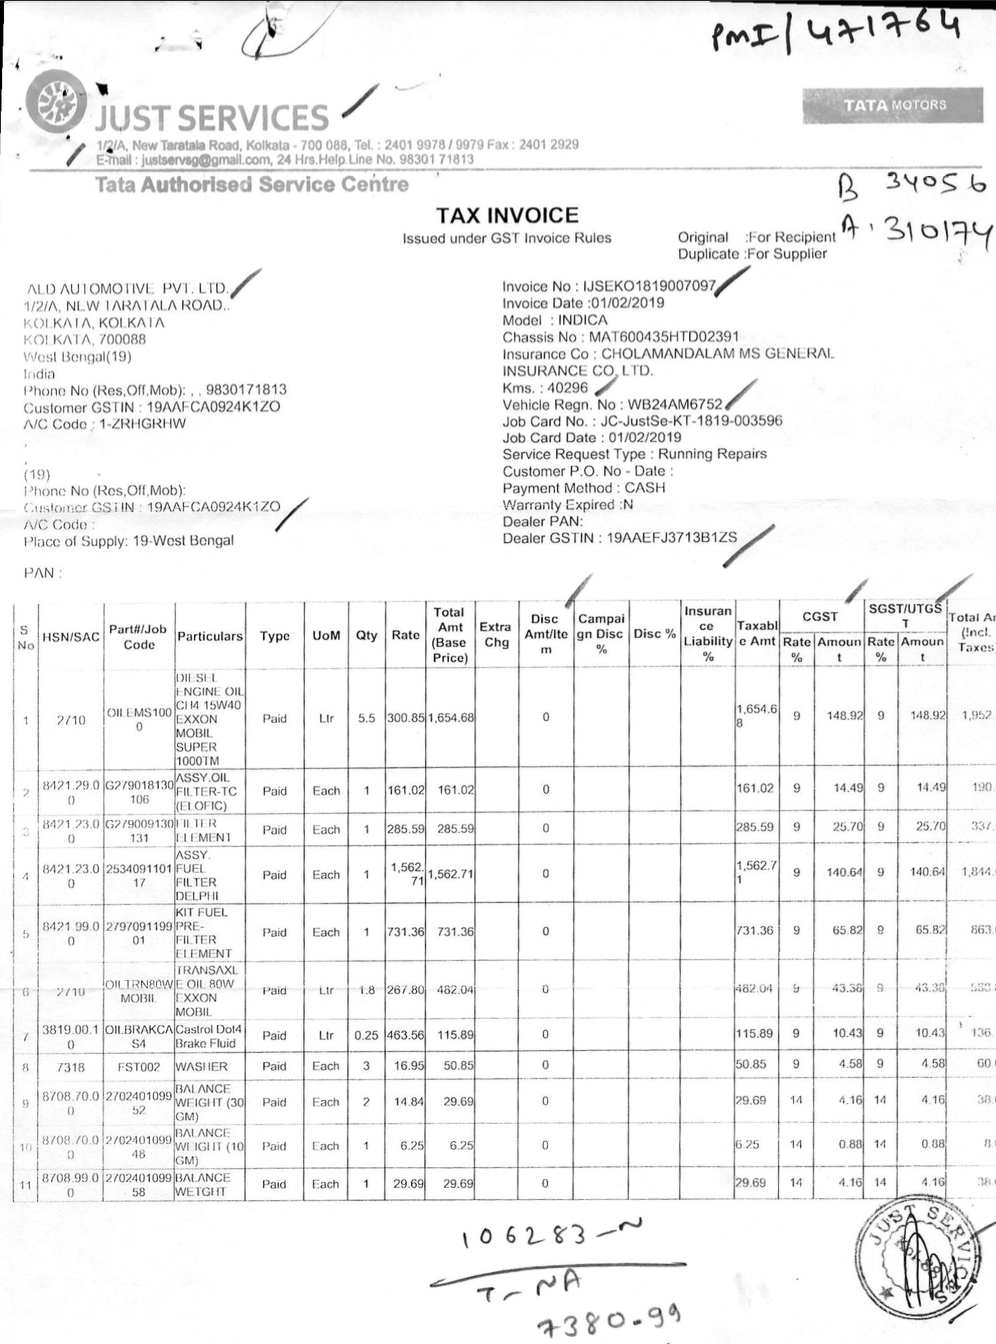
\includegraphics[width=0.45\textwidth]{graphics/bad_qual.png}
    \hfill % This adds space between the images
    % Include the second image
    \hfill % This adds space between the images
    % Include the third image
    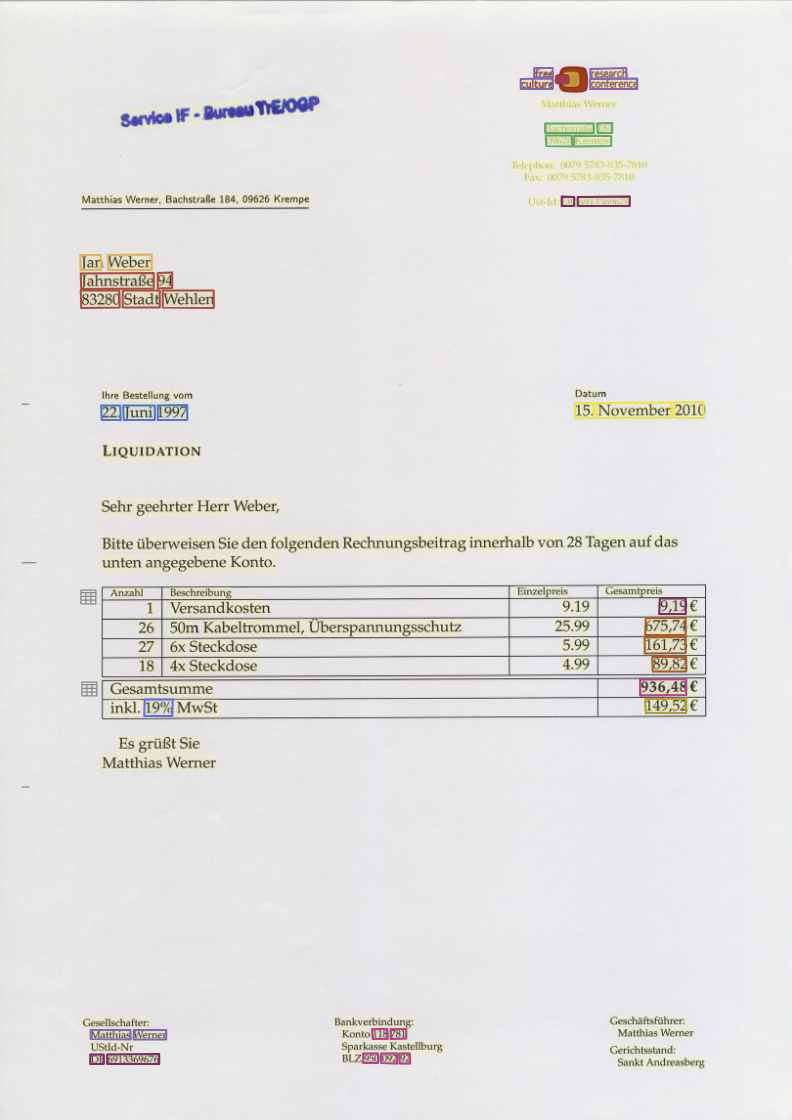
\includegraphics[width=0.45\textwidth]{graphics/doc_with_boc.png}
    \caption{Links: Beispiel für schlechte Qualität. Rechts: Beispiel für ein Dokument mit Bounding-Boxen und anderem Layout.}
    \label{fig:three_images}
  \end{figure}

Abbildung \ref{fig:three_images} zeigt, wie Layouts voneinander abweichen können. Links ist eine Rechnung mit einer vergleichsweise unübersichtlichen Tabelle zu sehen. Es gibt zudem viele händische Einträge. Die Rechnung in der Mitte ist deutlich übersichtlicher und strukturierter in Bezug auf das Layout. Die Rechnungen sind in unterschiedlichen Formaten und Layouts verfasst, um die Robustheit der Modelle zu testen. Die Rechnungen enthalten sowohl strukturierte als auch unstrukturierte Daten. Die strukturierten Daten umfassen beispielsweise Rechnungsnummer, Rechnungsdatum, Lieferdatum, Steuernummer, Umsatzsteuer-ID, IBAN, BIC, Gesamtbetrag, Steuersatz, Steuerbetrag, Netto- und Bruttobetrag. In Abb. \ref{fig:three_images} ist rechts ebenfalls eine Rechnung mit erkannten Daten zu sehen. Die farbigen Felder stellen die Bounding-Boxen der Felder dar. Die unstrukturierten Daten umfassen beispielsweise die Rechnungsadresse, die Lieferadresse, die Positionen, die Menge, die Einheit, den Preis und die Beschreibung. Die Rechnungen enthalten auch Logos, Werbung und andere Informationen, die nicht relevant sind. Diese müssen vor der Verarbeitung entfernt werden.

Der Prozess der Verarbeitungspipeline wird in Abb. \ref{fig:pipeline} dargestellt. Anders als üblicherweise empfohlen, erfolgt die Datenbereinigung in dieser Arbeit erst nach der ersten Verarbeitung. \footcites[Vgl. dazu ausführlich][]{wirth_crisp-dm_2000} Die initiale Phase umfasst die Annotation der Daten. Aufgrund begrenzter Ressourcen wird hierfür das Azure Document Intelligence Studio mit einem Custom Model genutzt, das speziell darauf ausgelegt ist, die Rechnungen zu labeln. Azure wird insbesondere wegen der begrenzten zeitlichen Ressourcen eingesetzt, da nicht genügend Zeit zur Verfügung steht, um die Daten händisch zu annotieren. Die Entscheidung für Azure und die sich daraus ergebenden Implikationen werden in einem späteren Kapitel diskutiert. Azure verwendet als OCR-Engine die proprietäre Microsoft Read OCR. Diese ist u. a. mit KI-Modellen verbessert worden, um bessere Ergebnisse im Bereich des \ac{Vrdu} zu erzielen. Ein Beispiel einer vollständig gelabelten Datei kann Anhang x entnommen werden. Es wird unterschieden zwischen Labeling-Verfahren für OCR-abhängige Modelle und solche, die unabhängig davon agieren. Für die unabhängigen Modelle werden keine Bounding-Boxen inkludiert. Bei Bounding-Boxen handelt es sich um vier Koordinaten in einem Dokument, die ein Rechteck um ein Wort oder eine Zeile bilden. Diese Bounding-Boxen sind notwendig, um die Position der Wörter im Dokument zu bestimmen (s. als Beispiel Abb. \ref{fig:three_images}). 

\begin{figure}[]
    \centering
    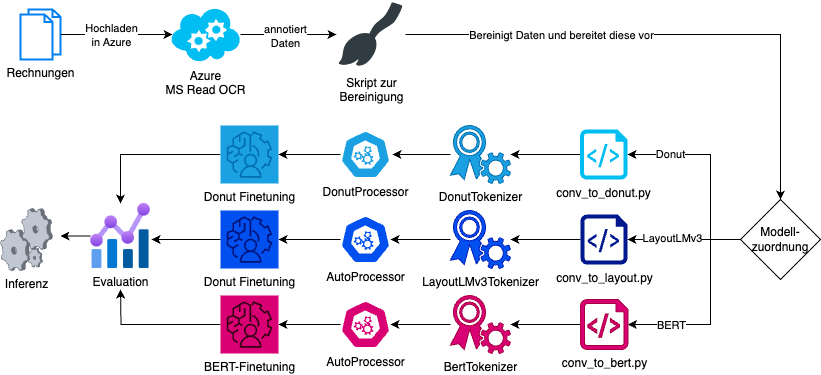
\includegraphics[width=160mm]{graphics/verarbeitungspipeline.png}
    \caption[Finetuning-Pipeline]{Finetuning-Pipeline}
    \label{fig:pipeline}
\end{figure}

Nach der Annotation werden aus dem Datensatz alle Dokumente, die keine Rechnungen sind oder einzelne Seiten dieser entfernt. Dies könnte zum Beispiel die letzten Seiten einer Rechnung betreffen, die Werbeslogans oder Verweise auf den Webshop enthalten. Die Aufbereitung der Daten unterscheidet sich je nach Modell. Während für LayoutLMv3 die Daten aus JSON in Listen umgewandelt und Bounding-Boxen normalisiert werden müssen, können die Daten für Donut im JSON-Format verbleiben. Ein Beispielhaftes JSON, welches  für das Training von aufbereitet wurde, Donut kann Abbildung x entnommen werden. In der Inferenz von Donut wird erwartet, dass die Informationen in diesem JSON-Format wieder ausgegeben werden.

\begin{figure}[]
    \centering
    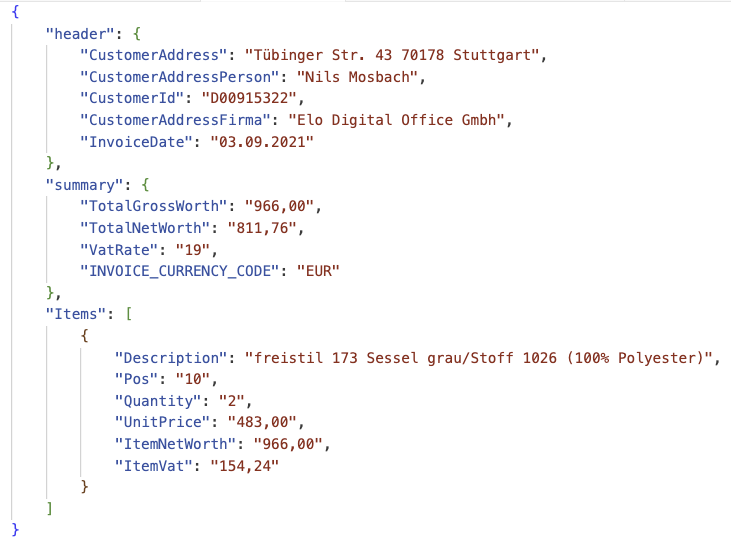
\includegraphics[width=100mm]{graphics/json-example.png}
    \caption[Beispielhaftes JSON]{Beispielhaftes JSON}
    \label{fig:json_example}
\end{figure}

Allerdings erfordert dies ein Mapping zwischen jedem JSON und dem zugehörigen Bild der Rechnung im Verzeichnis. Die nachfolgende Tokenisierung wird für alle drei Modelle mit modellspezifischen Tokenizern durchgeführt. Für die Erzeugung der Embeddings wird ebenfalls modellspezifisch vorgegangen, wobei jeder Modelltyp einen spezifischen Processor benötigt. Beim Processor handelt es sich um eine Klasse, die die Daten in ein für das Modell verständliches Format von Token Embeddings umwandelt.

Nach der Erzeugung der Embeddings durchlaufen die Modelle das Feintuning. Abgeschlossen wird dieser Prozess durch eine Evaluation mit 40 Rechnungen. In der abschließenden Inferenzphase wird das Modell mit einer Rechnung gefüttert, und die extrahierten Daten werden in einem strukturierten Format (in diesem Fall JSON) ausgegeben, was den gesamten Prozess der Verarbeitungspipeline abschließt.

\section{Besonderheiten von Donut in der Implementierung}
Das folgende Kapitel soll einen Überblick über die Gemeinsamkeiten und Unterschiede der Implementierung von Donut im Vergleich zu den anderen Modellen geben. Aus Gründen der Anschaulichkeit wird hierbei LayoutLMv3 als Vergleich verwendet. Die meisten Aspekte treffen jedoch auch auf das Modell BERT zu.

Bei der Gegenüberstellung der Finetuning-Pipelines für Donut und LayoutLMv3 fällt auf, dass die beiden Ansätze sowohl Gemeinsamkeiten als auch Unterschiede aufweisen, die jeweils für die spezifischen Anforderungen ihrer Modelle optimiert sind.

Es zeigen sich folgende Gemeinsamkeiten in der Implementierung: Beide Modelle verwendet spezialisierte Prozessoren (DonutProcessor für Donut und LayoutLMv3Processor für LayoutLMv3), um Bilder und Textdaten entsprechend vorzubereiten. Zusätzllich muss bei beiden Modellen auf die gründliche Bereinigung und Vorbereitung der Trainingsdaten gelegt werden. Bereits ein fehlerhaftes Dokument in den Trainingsdaten kann zu einer schlechten Performance der Modelle führen oder das Finetuning als Ganzes verhindern. Beide Modelle verwenden individuelle Trainingsdatensätze, die speziell darauf ausgerichtet sind, die für das jeweilige Modell erforderlichen Informationen zu verarbeiten und bereitzustellen. Die Eingangsdaten sind für alle Modelle dieselben. Sie unterscheiden sich lediglich in ihrer Aufbereitung. Die Trainingskonfiguration ist für beide Modelle dieselbe. Dazu gehören beispielsweise die Anzahl an Trainingsepochen, die Anzahl an Validierungen pro Epoche und die Trainingsschrittgröße. In einem späteren Kapitel wird im Detail auf die Trainingskonfiguration bzw. die Hyperparameter eingegangen. Für die grundlegende Gegenüberstellung bleiben sie jedoch gleich.

In der Verarbeitungspipeline für Donut werden dennoch mehr Unterschiede zu LayoutLMv3 als Gemeinsamkeiten deutlich. Den ersten maßgeblichen Unterschied bildet der Zugriff auf die Datensätze. Für die Verarbeitungspipeline von Donut war es notwendig, die Daten in einem speziellen Format zu speichern, das für das Modell geeignet ist. Daher wurde eine eigens entwickelte Dataset-Klasse(DonutDataset) verwendet, die speziell für die Verarbeitung und das Handling von Bild- und Textdaten entwickeltet wurde. Sie hat den Vorteil, dass die annotierten Daten im JSON Format nicht weiter transformiert werden müssen. Es braucht lediglich ein Mapping zwischen dem Bild, welches annotiert wurde und dem zugehörigen JSON. LayoutLMv3 greift auf bestehende Funktionalitäten der HuggingFace dataset-Bibliothek zurück. Hier müssen die Daten viel aufwendiger in eine Reihe von Listen bestehden aus \emph{Tokens, Bounding-Boxen, Labeln und Bildern} umgewandelt werden. Bounding-Boxen müssen zusätzlich normalisiert werden, was den Rechenaufwand nochmals linear erhöht. Bei Donut wird zudem auf eine differenzierte Annotation der Daten Wert gelegt, wobei layoutbasierte Informationen wie die zuvor genannten Bounding-Boxen nicht inkludiert werden. Dies führt zu einer einfacheren und schnelleren Annotation der Daten. Ein weiterer Unterschied besteht in der Tokenisierung und Eingabeverarbeitung. Die in dieser Arbeit entwickelte Donut-Pipeline umfasst spezielle Schritte zur Tokenisierung und Eingabeverarbeitung, die an das Design und die Anforderungen des Donut-Modells angepasst sind. LayoutLMv3 nutzt hingegen den AutoProcessor für eine automatisierte Verarbeitung, basierend auf dem Modellcheckpoint. Der AutoProcessor lädt für das jeweilige Modell den benötigten Processor automatisch. Schlussendlich zeigen sich bedeutende Unterschiede im Trainigns- und Evaluationssetup. Während Donut spezifische Klassen und Funktionen für das Training und die Evaluation implementiert, einschließlich angepasster Callbacks und einer umfangreichen Konfiguration, folgt LayoutLMv3 einem standardisierten Trainings- und Evaluationsprozess, der auf den HuggingFace-Trainings- und Evaluationsfunktionen basiert.

Die im Rahmen dieser Arbeit entwickelte Donut-Pipeline zeichnet sich v. a. durch zwei besondere Merkmale aus:
\begin{itemize}
    \item \textbf{Flexibilität in der Datenverarbeitung:} Die Donut-Pipeline zeichnet sich durch eine hohe Flexibilität bei der Aufbereitung und Anpassung der Trainingsdaten aus, um die Anforderungen des Modells optimal zu erfüllen.
    \item \textbf{Erweiterte Tokenisierung und Spezialtokens:} Die Donut-Pipeline beinhaltet spezielle Schritte zur Erweiterung der Tokenisierung und zur Integration von Spezialtokens, die für das Training und die Generierung von Vorhersagen entscheidend sind.
\end{itemize}

Insgesamt zeigt der Vergleich, dass beide Pipelines spezifisch für die Bedürfnisse und die Architektur der jeweiligen Modelle entwickelt wurden, mit besonderem Fokus auf die Optimierung der Datenvorbereitung, des Trainings und der Evaluation. Die Donut-Pipeline sticht durch ihre spezialisierte Herangehensweise und Anpassungsfähigkeit hervor, während die LayoutLMv3-Pipeline auf bewährte Methoden und Werkzeuge setzt, um eine effiziente Modellanpassung zu ermöglichen. Tabellen \ref{tab:donut_layoutlmv3_comparison} stellt die Unterschiede und Gemeinsamkeiten der Finetuning-Pipelines von Donut und LayoutLMv3 übersichtlich gegenüber.

Es ist wichtig hervorzuheben, dass es bedeutend Aufwendiger ist, eine Pipeline für Donut zu entwickeln, als für LayoutLMv3 oder BERT. Die beiden Referenzmodelle sind deutlich robuster im Hinblick auf das Preprocessing und die Eingabedaten. Dies kann dadurch erklärt werden, dass es sich bei BERT um ein bereits sehr etabliertes Modell handelt und LayoutLMv3 zusätzlich von Microsoft entwickelt wurde und daher auf eine Vielzahl von Ressourcen zurückgreifen kann. Donut hingegen ist ein relativ neues Modell, das noch nicht so weit verbreitet ist. Es handelt sich um ein offenes, nicht proprietäres Modell, das von einer kleinen Gruppe von Entwicklern entwickelt wurde. Daher ist es notwendig, eine spezialisierte Pipeline zu entwickeln, um das Modell optimal zu nutzen.

\begin{table}[ht]
    \centering
    \begin{tabularx}{\textwidth}{@{}lXX@{}}
    \toprule
    \textbf{Aspekt} & \textbf{Donut} & \textbf{LayoutLMv3} \\
    \midrule
    Spezialisierte Prozessoren & Verwendet DonutProcessor & Verwendet LayoutLMv3Processor \\
    Datenbereinigung & Hohe Flexibilität bei der Datenvorbereitung & Erfordert umfangreiche Datenbereinigung und -vorbereitung \\
    Trainingsdatensätze & Verwendet eine speziell entwickelte Dataset-Klasse (DonutDataset) & Greift auf bestehende Funktionalitäten von Hugging Face zurück \\
    Annotation der Daten & Differenzierte Annotation ohne Bounding Boxes für layoutbasierte Informationen & Verwendet detaillierte Annotationen inklusive Bounding Boxes \\
    Tokenisierung & Spezielle Schritte zur Tokenisierung und Eingabeverarbeitung, angepasst an das Modell & Nutzt den AutoProcessor für automatisierte Verarbeitung \\
    Trainings- und Evaluationssetup & Implementiert spezifische Klassen und Funktionen für das Training und die Evaluation & Folgt einem standardisierten Trainings- und Evaluationsprozess \\
    \bottomrule
    \end{tabularx}
    \caption{Vergleich der Finetuning-Pipelines von Donut und LayoutLMv3}
    \label{tab:donut_layoutlmv3_comparison}
\end{table}
    

\section{Diskussion der Implementierung}
Eine umfassende Diskussion und kritische Betrachtung der vorliegenden Bachelorarbeit erfolgt in Kapitel 6. Dennoch soll der folgende Abschnitt eine kruze Diskussion der Implementierung der Modelle und der Verarbeitungspipelines bieten. Damit sollen einige Entscheidungen erläutert werden und die Gründe für die gewählten Vorgehensweisen dargelegt werden.

Die im vorherigen Abschnitt erläuterten Besonderheiten der Donut-Pipeline treffen nicht zwingend auf jede Donut-Pipeline zu. Die Implementierung der Donut-Pipeline in dieser Arbeit wurde speziell auf die Anforderungen des Modells und die verfügbaren Ressourcen zugeschnitten. Des weiteren erfolgte die Implementierung unter der Annahme, das Modell in der Endanwendung bei ausreichend guten Ergebnissen einzusetzen. Daher wurde hier der Fokus auf die Optimierung von Donut gelegt. Hiermit lassen sich auch die Flexibilität der Datenverarbeitung und die erweiterte Tokenisierung und Spezialtokens erklären. Die Implementierung der LayoutLMv3- und BERT-Pipeline hingegen erfolgte unter der Annahme, dass die Modelle nur als Vergleichsmodelle dienen soll. Daher wurde hier auf bewährte Methoden und Werkzeuge zurückgegriffen, um eine effiziente Modellanpassung zu ermöglichen. Die Implementierung der BERT-Pipeline erfolgte unter der Annahme, dass das Modell als Backup-Modell für Donut dienen soll. Daher wurde hier auf eine effiziente Implementierung geachtet, die eine schnelle Anpassung und Integration in die Endanwendung ermöglicht. Die im vorgegangen Abschnitt implizierten Vorteile können zu großen Teilen auch auf die anderen Pipelines übertragen werden. Da die Vergleichsmodelle jedoch nur zu Forschungszwecken eingesetzt werden, wurde hier auf eine spezialisierte Implementierung, d. h. auf eine, die unter Umständen in der Endanwendung verwendet werden könnte, verzichtet.

Eine Schwachstelle der Implementierung ist die Verwendung vom Azure Docuement Intelligence Studio für die Annotation der Daten. Azure bietet zwar eine schnelle und effiziente Möglichkeit, die Daten zu annotieren, jedoch ist das Format stellenweise nicht passend für die Weiterverarbeitung in Transformern angepasst. Für LayoutLMv3 gibt Azure auch Bounding-Boxen bei der Annotation zurück. Diese sind jedoch in Zoll formatiert. Daher ist noch die Transformation aller Größen in Pixeln notwendig. Dies führt zu einem erhöhten Rechenaufwand und einer längeren Verarbeitungszeit. Ein weiterer Nachteil ist die Abhängigkeit von Azure. Sollte Azure nicht verfügbar sein, wäre die automatisierte Annotation der Daten mittels vortrainierter Modelle nicht möglich. Diese Form der Annotation nutzt maschinelle Lernmodelle, die auf der Azure-Plattform gehostet werden, um Textelemente in den Dokumenten zu erkennen und entsprechend zu klassifizieren. Der Einsatz solcher Modelle verursacht Rechenaufwand, da jede Annotation eine Vorhersage durch das Modell erfordert, welches rechenintensive Prozesse wie das Laden des Modells, die Verarbeitung der Eingabedaten und die Ausführung der inferentiellen Algorithmen umfasst. Sollte Azure nicht verfügbar sein, wäre die automatisierte Annotation der Daten mittels vortrainierter Modelle nicht möglich. Diese Form der Annotation nutzt maschinelle Lernmodelle, die auf der Azure-Plattform gehostet werden, um Textelemente in den Dokumenten zu erkennen und entsprechend zu klassifizieren. Der Einsatz solcher Modelle verursacht Rechenaufwand, da jede Annotation eine Vorhersage durch das Modell erfordert, welches rechenintensive Prozesse wie das Laden des Modells, die Verarbeitung der Eingabedaten und die Ausführung der inferentiellen Algorithmen umfasst.

\chapter{Ergebnisse}
In Kapitel 5 werden die Ergebnisse der durchgeführten Experimente dargelegt, welche die Effizienz und Genauigkeit von Document Understanding Transformers, insbesondere des Donut-Modells, im Vergleich zu traditionellen OCR-basierten Modellen und LayoutLMv3 evaluieren. Die Auswertung basiert auf den zuvor definierten Metriken: Accuracy, F1-Score und GPU-Stunden (GPUh), die eine umfassende Einsicht in die Leistungsfähigkeit der untersuchten Modelle unter realen Anwendungsbedingungen ermöglichen. Die im folgenden Kapitel präsentierten Ergebnisse und Beobachtungen sind, sofern nicht anders angegeben, Eigenleistung dieser Arbeit. Sie basieren auf den Experimenten, die mit den drei Modellen Donut, LayoutLMv3 und BERT im Rahmen dieser Bachelorarbeit durchgeführt wurden. Fremde Beobachtungen und Ergebnisse sind entsprechend gekennzeichnet.

Die Analyse der Ergebnisse beginnt mit einer detaillierten Bewertung der Modellperformance, fokussiert auf Accuracy und F1-Score. Diese Metriken spiegeln wider, wie präzise die Modelle relevante Informationen aus den Dokumenten extrahieren und Fehlinterpretationen minimieren. Es wird aufgezeigt, inwiefern das Donut-Modell seine Stärken gegenüber den herkömmlichen OCR-Systemen und LayoutLMv3 ausspielen konnte, insbesondere bei der Verarbeitung heterogener Datensätze aus dem Unternehmensumfeld. Des Weiteren wird der Einfluss der Datenmenge und -qualität auf die Modellperformance diskutiert, um zu verdeutlichen, wie diese Faktoren die Effizienz und Genauigkeit der Informationsgewinnung beeinflussen.

\section{Detailierte Ergebnisspräsentation}
Zunächst sollen in folgendem Abschnitt die besten Ergebnisse der Modellperformance in Bezug auf die Metriken Accuracy, F1-Score und GPUh präsentiert werden. Die Ergebnisse basieren auf den Experimenten, die mit den drei Modellen Donut, LayoutLMv3 und BERT durchgeführt wurden. Die Resultate der Modellperformance sind in Tabelle \ref{tab:best_results} zusammengefasst.
\begin{table}[h]    
\centering
    \begin{tabularx}{\textwidth}{lXXX}
      \toprule
      & \textbf{Donut} & \textbf{LayoutLMv3} & \textbf{BERT}  \\
      \midrule
      F1 Score & 80.2 & \textbf{92.1} & 91.1 \\
      \addlinespace
      Accuracy & 85.7 & \textbf{94.1} & 93.9 \\
        \addlinespace
        GPUh & 3.11 & 2.04 & \textbf{0.077} \\
      \bottomrule
    \end{tabularx}
    \caption{Beste Ergebnisse der Modellperformance (Epochen: 20, Schrittmenge: 100, Per-Device Train/Eval Batch-Size: 2, Evaluation: Alle 3 Epochen, Metrik für das beste Modell: F1, Learnrate: 3e-5)}
    \label{tab:best_results}
\end{table}
Es wird ersichtlich, dass Donut in keiner der Metriken die besten Ergebnisse erzielen konnte. LayoutLMv3 hingegen konnte sowohl den höchsten F1-Score als auch die höchste Accuracy erreichen. BERT hingegen benötigte die wenigsten GPU-Stunden, um die Dokumente zu verarbeiten. 

Vor der Interpretation der Ergebnisse ist hervorzuheben, dass die Leistung des Donut-Modells hinsichtlich der Accuracy und des F1-Scores mit Werten zwischen 80-85 \% durchaus zufriedenstellend ist und nahe an den in der Originalpublikation berichteten Ergebnissen liegt. \footcites[Vgl.][]{kim_ocr-free_2021} Da Donut v. a. auf englischen Daten trainiert wurde ist die Modellperformance auf deutschen Datensätzen etwas schlechter. Die Layouts von bspw. Rechnungen oder Lieferscheinen können sich in Deutschland von denen in den USA unterscheiden. Des weiteren ist anzumerken, dass das Finetuning mit 180, 300, 850 Trainingsdaten stattgefunden hat. Dies ist deutlich weniger als der Inhalt von \ac{CORD} oder \ac{FUNSD}. Diese Situation ist für die Studie vorteilhaft, da sie die tatsächliche Verfügbarkeit von Trainingsdaten in einem Unternehmen realistisch darstellt. Allerdings begrenzt sie auch das mögliche Leistungsspektrum von Donut. Zwar beschäftigt sich die vorliegende Bachelorarbeit mit der Frage, ob Donut den Prozess der Dokumentenverarbeitung effizienter und genauer gestalten kann, jedoch sollen die Referenzergebnisse von LayoutLMv3 und BERT nicht außer Acht gelassen werden, da diese ebenfalls Implikationen für die beteiligten Prozesse der Dokumentenverarbeitung haben. Potenziell könnte sich hier für Unternehmen eine Alternative zu Donut ergeben, die ebenfalls effizient und genau arbeitet.

Der niedrige F1-Score von 80 \% bei Donut deutet darauf hin, dass bei jeder fünften Vorhersage ein Fehler in der Extraktion einer Entität gemacht wird. Dies kann aus zwei Perspektiven gedeutet werden. Einerseits bedeutet es für die vollständige Automatisierung, dass regelmäßig händisch Fehlerkorrekturen vorgenommen werden müssen. Ein niedriger F1-Score für das Donut-Modell bedeutet, dass das Modell Schwierigkeiten hat, relevante Informationen aus Dokumenten effektiv zu identifizieren und zu extrahieren. Für Anwendungsfälle, in denen es kritisch ist, präzise und vollständige Informationen aus Dokumenten zu extrahieren, könnte ein niedriger F1-Score des Donut-Modells bedeuten, dass das Modell möglicherweise nicht die gewünschte Effektivität erreicht. Dies könnte zu einer erhöhten Nachbearbeitungszeit führen, um Fehler zu korrigieren oder fehlende Informationen manuell zu ergänzen, was den Automatisierungsgrad und die Effizienz der Dokumentenverarbeitung reduziert. Andererseits bedeutet es, dass in manuellen Arbeitsfeldern lediglich jeder fünfte Eintrag von einer Person nachbereitet werden muss. In Umfeldern, in denen noch keine Automatisierung besteht, kann Donut daher eine kostengünstige Alternative bieten, um Mitarbeiter in der Dokumentenverarbeitung zu entlasten.

Die Accuracy von rund 85 \% beim Donut-Modell bedeutet, dass ein signifikanter Anteil der vom Modell getroffenen Vorhersagen über das gesamte Spektrum möglicher Klassen (z. B. relevante Informationen, irrelevante Informationen, verschiedene Arten von Informationen etc.) falsch ist. Auch im Hinblick auf die Accuracy ist es wichtig, die Ergebnisse von Donut im Kontext der spezifischen Anforderungen und Anwendungsfälle zu interpretieren, um zu beurteilen, ob das Modell die gewünschte Genauigkeit und Zuverlässigkeit bietet. Im Falle der Implementierung von Donut in der Endanwendung würde die niedrige Accuracy bedeuten, dass das Modell eine beträchtliche Anzahl von Fehlern bei der Informationsgewinnung macht, was die händische Nachbearbeitung und Korrektur von Dokumenten erfordert. Bei solch einer hohen Anzahl an Fehlern ist jedoch fraglich, ob der Einsatz von Donut tatsächlich zu einer Effizienzsteigerung führen würde, da die manuelle Nachbearbeitung einen erheblichen Zeitaufwand erfordert und die Vorteile der Automatisierung zunichtemacht.

Auch im Hinblick auf die Effizienz (GPUh) konnte Donut nicht besser abschneiden als die Referenzmodelle. Mit 3.11 GPU-Stunden benötigt Donut mehr als das 40-fache an Rechenleistung als BERT, um die Dokumente zu verarbeiten. Dies ist ein deutlicher Hinweis darauf, dass Donut nicht nur in der Modellperformance, sondern auch in der Effizienz hinter den Referenzmodellen zurückbleibt. Die hohe Anzahl an GPU-Stunden, die Donut benötigt, um die Dokumente zu verarbeiten, bedeutet, dass das Modell sehr rechenintensiv ist und eine erhebliche Menge an Rechenressourcen in Anspruch nimmt. Es sei gesagt, dass BERT kein layoutbasiertes Modell ist und beim Training keine Bilder verarbeiten muss. Nichtsdestotrotz hat LayoutLMv3 ebenfalls eine viel höhere Effizienz als Donut. Diese Zahlen müssen jedoch im Kontext betrachtet werden. Zwar benötigt Donut mehr GPU-Stunden als die Referenzmodelle, jedoch ist die Anzahl an GPU-Stunden insgesamt sehr gering. Die Kosten für die Rechenleistung von Donut in der Rechenumgebung beliefen sich bei einem Trainingsdatensatz von 850 Dokumenten, einer Schrittmenge von 100 und 30 Epochen auf 18,36 \$. Dies ist ein sehr geringer Betrag, der in den meisten Unternehmen keine signifikante Rolle spielen sollte.

\section{Ergebnisinterpretation und Implikationen}
Die Ergebnisse der Modellperformance zeigen, dass Donut im Vergleich zu den Referenzmodellen LayoutLMv3 und BERT in den Metriken Accuracy, F1-Score und Effizienz (GPUh) nicht die besten Ergebnisse erzielen konnte. Es gilt nun zu untersuchen, welche Faktoren einen Einfluss auf die Modellperformance haben, um so die in Kapitel 3 aufgestellten Hypothesen zu überprüfen und die Forschungsfrage zu beantworten.

Der wohl entscheidendste Faktor ist die Größe und Qualität des Datensatzes. Donut wurde mit 180, 300 und 850 Trainingsdaten trainiert. Die Graphen in Abbildung \ref{fig:experiment_results} zeigen, wie sich die Datensatzgröße auf die Metriken auswirkt. Bei Donut zeigt sich im Vergleich zu seinen Konkurrenten, dass es eine viel höhere Menge an Daten braucht, um die Modellperformance so weit zu steigern, dass Donut mehr Felder richtig erkennt als nicht. Dies ist ein Hinweis darauf, dass Donut eine hohe Menge an Trainingsdaten benötigt, um seine volle Leistungsfähigkeit zu entfalten. Dies ist ein wichtiger Aspekt, der bei der Implementierung von Donut in Betracht gezogen werden sollte, da die Verfügbarkeit von Trainingsdaten in der Praxis oft begrenzt ist. 
    
Die Qualität der Trainingsdaten ist ebenfalls ein wichtiger Faktor, der die Modellperformance beeinflusst. Wie in Kapitel 3 beschrieben, wurden die Trainingsdaten in diesem Experiment von einem leistungsfähigen Extraktionstool in Azure annotiert. BERT und LayoutLMv3 wurden mit den gleichen Daten trainiert. Es wird deutlich, dass die beiden OCR-abhängigen Modelle mit viel weniger Daten gute Ergebnisse präsentieren. Im Experiment wurde deutlich, dass LayoutLMv3 und BERT einen F1-Score über 80 \% mit lediglich 180 Daten erzielen konnten, während Donut lediglich 13 \% erreichte (Vgl. dazu Abb. \ref{fig:experiment_results} und Tab. \ref{tab:donut_metrics}).Eine genauere Betrachtung im Training zeigt, dass die OCR-abhängigen Modelle viel weniger Daten brauchen, um die gewünschten Labels zu lernen. Bspw. kann LayoutLMv3 auch untrainiert Felder schon an den richtigen Positionen erkannt haben. Die Vorhersage entsprach jedoch noch nicht dem Label, gegen welches geprüft wurde. Ein Beispiel wäre, dass LayoutLMv3 auch untrainiert, ein Lieferdatum in einem Dokument erkennt, aber dieses nicht als \emph{Lieferdatum} annotiert, sondern als \emph{Delivery Date}. Das passiert, da das Modell ursprünglich auf englischen Daten trainiert wurde. Zwar wäre das Feld fachlich gesehen richtig erkannt gewesen. Jedoch würde bei der Prüfung gegen die zugrunde liegende Ground Truth das Feld als falsch gewertet werden, da es nicht spezifisch \emph{Lieferdatum} heißt. Bei den OCR-abhängigen Modellen verschwindet dieser Effekt schon bei sehr wenigen Daten. Donut hingegen benötigt jedoch mehr als 200 Trainingsdaten, um die Labels zu lernen.

\pgfplotsset{compat=1.9}

\begin{figure}
\centering
% F1 Score
\begin{minipage}{.32\textwidth}
\begin{tikzpicture}
\begin{axis}[
    title={F1 Score},
    xlabel={Datensatzgröße},
    ylabel={F1},
    xmin=180, xmax=850,
    ymin=0, ymax=1,
    xtick={180,300,850},
    ytick={0,0.25,0.5,0.75,1},
    tick label style={font=\tiny},
    label style={font=\small},
    title style={font=\small},
    legend style={font=\tiny},
    legend pos=south east,
    ymajorgrids=true,
    grid style=dashed,
    width=\linewidth, height=6cm,
]

\addplot[color=blue,mark=*,] coordinates {(180,0.133)(300,0.649)(850,0.802)};
\addlegendentry{Donut}

\addplot[color=red,mark=*,] coordinates {(180,0.818)(300,0.909)(850,0.921)};
\addlegendentry{LayoutLMv3}

\addplot[color=green,mark=*,] coordinates {(180,0.846)(300,0.911)(850,0.884)};
\addlegendentry{BERT}

\end{axis}
\end{tikzpicture}
\end{minipage}%
%
% Accuracy
\begin{minipage}{.32\textwidth}
\begin{tikzpicture}
\begin{axis}[
    title={Accuracy},
    xlabel={Datensatzgröße},
    ylabel={Acc},
    xmin=180, xmax=850,
    ymin=0, ymax=1,
    xtick={180,300,850},
    ytick={0,0.25,0.5,0.75,1},
    tick label style={font=\tiny},
    label style={font=\small},
    title style={font=\small},
    legend style={font=\tiny},
    legend pos=south east,
    ymajorgrids=true,
    grid style=dashed,
    width=\linewidth, height=6cm,
]

\addplot[color=blue,mark=*,] coordinates {(180,0.245)(300,0.702)(850,0.857)};
\addlegendentry{Donut}

\addplot[color=red,mark=*,] coordinates {(180,0.875)(300,0.942)(850,0.941)};
\addlegendentry{LayoutLMv3}

\addplot[color=green,mark=*,] coordinates {(180,0.921)(300,0.939)(850,0.935)};
\addlegendentry{BERT}

\end{axis}
\end{tikzpicture}
\end{minipage}%
%
% GPU Stunden
\begin{minipage}{.32\textwidth}
\begin{tikzpicture}
\begin{axis}[
    title={GPUh},
    xlabel={Datensatzgröße},
    ylabel={GPUh},
    xmin=180, xmax=850,
    ymin=0, ymax=3.5,
    xtick={180,300,850},
    ytick={0,1,2,3},
    tick label style={font=\tiny},
    label style={font=\small},
    title style={font=\small},
    legend style={font=\tiny},
    legend pos=north west,
    ymajorgrids=true,
    grid style=dashed,
    width=\linewidth, height=6cm,
]

\addplot[color=blue,mark=*,] coordinates {(180,0.54)(300,1.382)(850,3.11)};
\addlegendentry{Donut}

\addplot[color=red,mark=*,] coordinates {(180,0.34)(300,0.59)(850,2.04)};
\addlegendentry{LayoutLMv3}

\addplot[color=green,mark=*,] coordinates {(180,0.053)(300,0.077)(850,0.255)};
\addlegendentry{BERT}

\end{axis}
\end{tikzpicture}
\end{minipage}
\caption{Vergleich der Modellmetriken F1 Score, Accuracy und GPU Stunden (GPUh) über verschiedene Datensatzgrößen.}
\label{fig:experiment_results}
\end{figure}


\newcolumntype{Y}{>{\centering\arraybackslash}X}

\begin{table}
\centering
\begin{tabularx}{\textwidth}{@{}lYYY@{}}
\toprule
& \textbf{Donut} & \textbf{LayoutLMv3/LMv3} & \textbf{BERT} \\
\midrule
\multicolumn{4}{c}{\textbf{180 Dataset} (126 Train, 27 Test, 27 Val)} \\
\midrule
F1         & 0.133 & 0.818 & 0.846 \\
Accuracy   & 0.245 & 0.875 & 0.921 \\
GPUh       & 0.54  & 0.34  & 0.053 \\
\midrule
\multicolumn{4}{c}{\textbf{300 Dataset} (240 Train, 30 Test, 30 Val)} \\
\midrule
F1         & 0.649 & 0.909 & 0.911 \\
Accuracy   & 0.702 & 0.942 & 0.939 \\
GPUh       & 1.382 & 0.59  & 0.077 \\
\midrule
\multicolumn{4}{c}{\textbf{850 Dataset} (730 Train, 40 Test, 80 Val)} \\
\midrule
F1         & 0.802 & 0.921 & 0.884 \\
Accuracy   & 0.857 & 0.941 & 0.935 \\
GPUh       & 3.11  & 2.04  & 0.255 \\
\bottomrule
\end{tabularx}
\caption{Vergleich von Modellen über verschiedene Datensätze}
\label{tab:donut_metrics}
\end{table}

Auffällig sind die sehr guten Ergebnisse von BERT. Gegenüber der bestehenden Forschung in der Literatur hat BERT in diesem Experiment mit einer sehr guten Performance überzeugt. \footcites[Vgl. dazu ausführlich][]{kim_ocr-free_2021}[][]{huang_layoutlmv3_2022} Da die Ergebnisse stark von denen in der bisherigen Literatur abweichen, müssen diese besonders kritisch betrachtet werden. BERT verfügt über keine Möglichkeit, Layoutinformationen zu verarbeiten. Es ist daher überraschend, dass BERT so gute Ergebnisse erzielt hat. Zunächst ist es wichtig zu verstehen, welche Informationen BERT beim Training als Input erhält. BERT erhält als Input die Texte der Dokumente. Der Datensatz hält zu jedem Token ein Label fest. Dies kann an folgendem Beispiel nachvollzogen werden: 

Eine Liste aus Tokens [Technik, GmbH, 13, 12, 2022] würde bspw. das Label [CompanyName, CompanyName, DateDay, DateMonth, DateYear] erhalten. BERT lernt also die Labels anhand der Tokens. 

Es ist daher nicht verwunderlich, dass BERT so gute Ergebnisse erzielt hat. BERT hat die Labels der Tokens gelernt und kann daher sehr gut die Labels neuen Texten zuordnen. Ein entscheidender Schwachpunkt ist jedoch, dass BERT vollständig vom Inputtext in der Inferenz abhängig ist. Eine schwache vorgelagerte OCR kann die Ergebnisse daher stark beeinflussen. 

Der Einfluss der OCR zeigt sich vor allem im Vergleich bei LayoutLMv3 zwischen Finetuning und Inferenz. Im Finetuning wurden Daten durch die vergleichsweise sehr genaue Microsoft Read OCR aufbereitet. In der Inferenz hingegen wurden die Daten durch Tesseract für die Verarbeitung vorbereitet. Abbildung \ref{fig:ocr_results} zeigt die Unterschiede in der Extraktion der beiden OCR-Systeme. Es wird deutlich, dass Microsoft Read OCR sehr viel genauere Ergebnisse liefert als Tesseract. Dies zeigt sich auch in den Ergebnissen von LayoutLMv3. Während LayoutLMv3 im Finetuning sehr gute Ergebnisse liefert, sind die Ergebnisse in der Inferenz deutlich schlechter. Das Selbe trifft für BERT zu. In diesem Experiment wurden mehrere genaue Analysen einzelner Rechnungen durchgeführt. Folgende Probleme entstanden im Beispiel von Abbildung \ref{fig:ocr_results} bei der Verwendung von Tesseract:
\begin{itemize}
    \item Nur die ersten beiden Teile der IBAN wurden erkannt.
    \item Ein nicht vorhandenes Bezahlt-Feld wurde fünf Mal erkannt.
    \item Der Mehrwertsteuersatz wurde sechs Mal erkannt.
    \item Ein nicht vorhandener Rabatt in Prozent wurde erkannt.
    \item Die nicht vorhandene Umsatzsteuer-ID wurde nicht erkannt.
    \item Das nicht vorhandene Land des Verkäufers wurde erkannt.
    \item Das Fälligkeitsdatum wurde zwei Mal erkannt.
    \item Alle weiteren Felder, die in Abbildung \ref{fig:ocr_results} links zu sehen sind, aber nicht rechts, wurden nicht erkannt.
\end{itemize}

\begin{figure}[]
    \centering
    % Include the first image with specific dimensions
    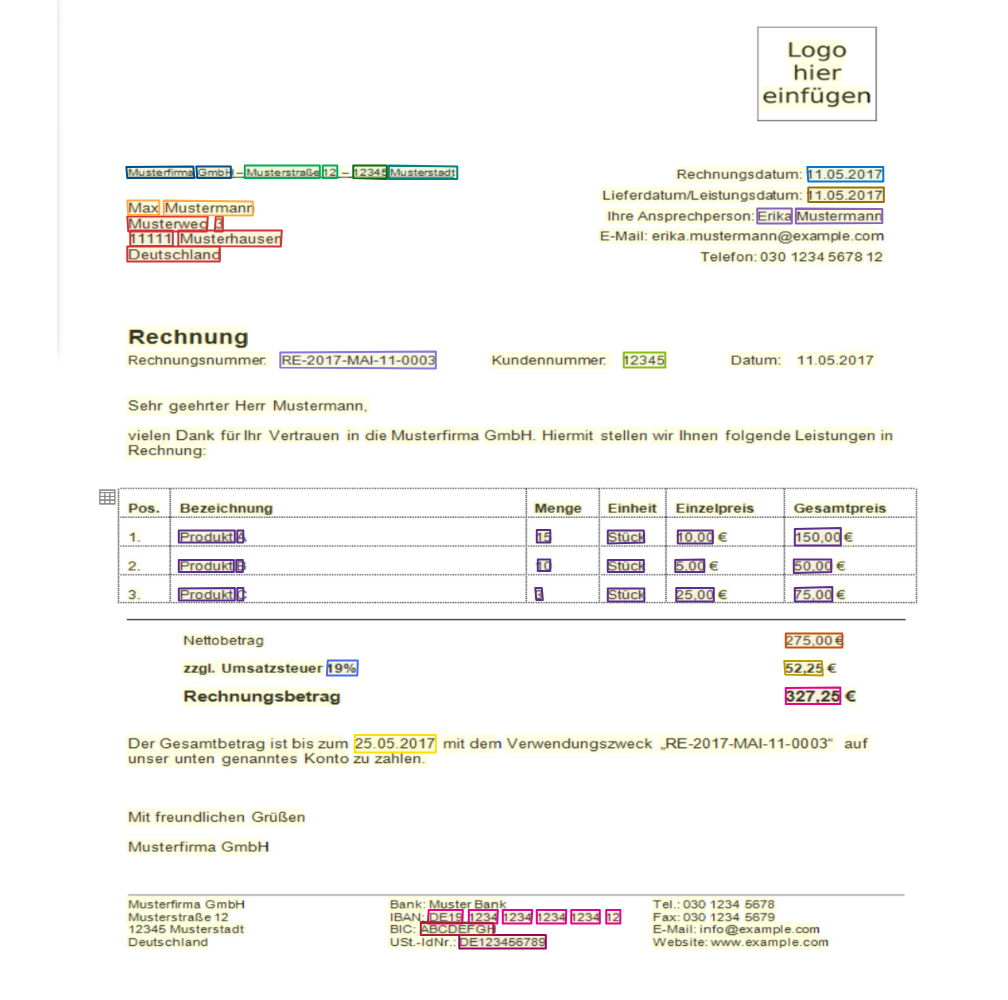
\includegraphics[width=0.45\textwidth,height=0.4\textheight,keepaspectratio=false]{graphics/ms_read.png}
    \hfill % This adds space between the images
    \hfill
    % Include the third image with specific dimensions
    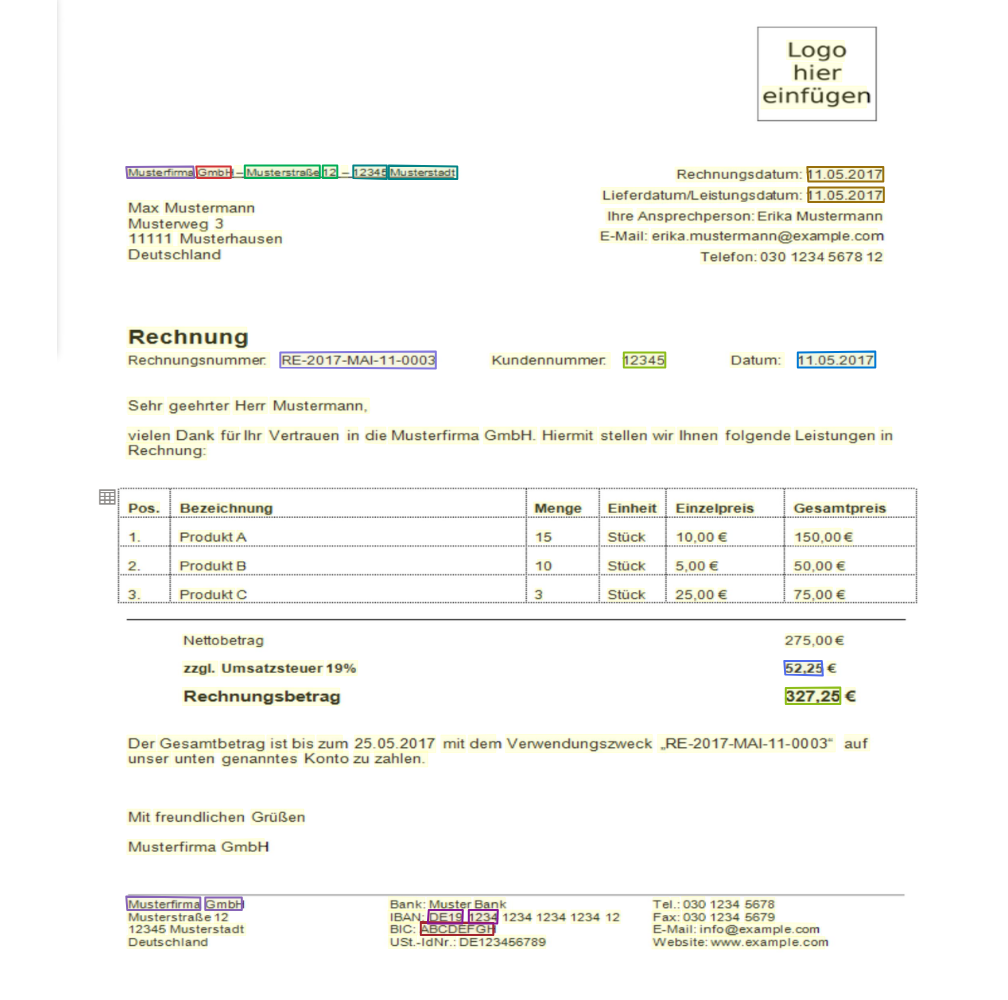
\includegraphics[width=0.45\textwidth,height=0.4\textheight,keepaspectratio=false]{graphics/tesseract.png}
    \caption{Links: Extraktion durch Microsoft Read OCR. Rechts: Extraktion durch Tesseract.}
    \label{fig:ocr_results}
\end{figure}

Des Weiteren müssen die niedrigen GPUh ebenso unter dem Umstand der Abwesenheit von jeglichen layoutbasierten Informationen betrachtet werden. BERT benötigt keine Bilder und kann daher sehr schnell arbeiten.

Tabelle \ref{tab:donut_metrics} zeigt die Metriken des Donut-Modells über verschiedene Datensatzgrößen. Es wird deutlich, dass die Modellperformance mit steigender Datensatzgröße zunimmt. Donut benötigt eine hohe Menge an Trainingsdaten, um die Labels zu lernen. Dies ist ein wichtiger Aspekt, der bei der Implementierung von Donut in Betracht gezogen werden sollte, da die Verfügbarkeit von Trainingsdaten in der Praxis oft begrenzt ist. Aus den Ergebnissen wird ebenfalls deutlich, dass die benötigten GPUh für das Modell mit steigender Datensatzgröße zunehmen. Auf der anderen Seite nimmt die Änderungsrate von F1-Score und Accuracy mit steigender Datensatzgröße ab. Dies bedeutet, dass das Modell mit steigender Datensatzgröße nicht mehr so stark an Performance gewinnt, wie es bei kleineren Datensätzen der Fall ist. Für Unternehmen ist es daher wichtig, die Kosten und den Nutzen von zusätzlichen Trainingsdaten abzuwägen, um eine effiziente und effektive Implementierung von Donut zu gewährleisten. Sicherlich gibt es hierfür auch andere Ansätze, wie bspw. das Training auf synthetischen Daten. Dieser Ansatz wurde jedoch in dieser Arbeit nicht weiter verfolgt. Für jedes Unternehmen gibt es wahrscheinlich eine optimale Datengröße, die die Kosten und den Nutzen von zusätzlichen Trainingsdaten ausbalanciert. Dies hängt jedoch davon ab, wie wichtig die Genauigkeit und Effizienz der Dokumentenverarbeitung für das Unternehmen sind. Daher kann diese Frage in dieser Arbeit nicht weiter verfolgt werden.

Die Ergebnisse zeigen, dass Donut in der Modellperformance hinter den Referenzmodellen zurückbleibt. Die Schwäche von Donut im Vergleich zu den Referenzmodellen ist der hohe Datenbedarf. Die Stärke von BERT liegt v. a. in seiner Leichtgewichtigkeit. Demgegenüber steht die Schwäche, dass BERT keine Layoutinformationen verarbeiten kann. LayoutLMv3 hingegen ist sehr gut in der Lage, Layoutinformationen zu verarbeiten. Von daher sind die sehr guten Ergebnisse von BERT dadurch zu erklären, dass die Daten von der ohnehin sehr performanten Microsoft Read OCR annotiert und verarbeitet wurden. 

\pgfplotsset{width=10cm,compat=1.9}

\begin{figure}[h]
    \centering
    \begin{tikzpicture}
    \begin{axis}[
        title={Accuracy von Donut über Datensatzgrößen},
        xlabel={Datensatzgröße},
        ylabel={Accuracy},
        width=0.45\linewidth,
        height=5cm,
        xmin=150, xmax=900,
        ymin=0, ymax=1,
        xtick={180,300,500,850},
        ytick={0.2, 0.4, 0.6, 0.8, 1.0},
        legend pos=south east,
        ymajorgrids=true,
        grid style=dashed,
    ]
    
    \addplot[
        color=blue,
        mark=*, % Markierungsstil
        thick, % Linienstärke
        ]
        coordinates {
        (180,0.245)(300,0.702)(500,0.835)(850,0.857)
        };
        \addlegendentry{Donut}
    
    \end{axis}
    \end{tikzpicture}
     % Platz für das zweite Diagramm
    \begin{tikzpicture}
    \begin{axis}[
        title={Accuracy von nach Kim et al. (2021)},
        xlabel={Datensatzgröße},
        ylabel={Accuracy},
        width=0.45\linewidth,
        height=5cm,
        xmin=60, xmax=820,
        ymin=50, ymax=100,
        xtick={80, 160, 400,800},
        ytick={50, 60, 70, 80, 90},
        legend pos=south east,
        ymajorgrids=true,
        grid style=dashed,
    ]
    
    \addplot[
        color=cyan,
        mark=*, % Markierungsstil
        thick, % Linienstärke
        ]
        coordinates {
        (80,79)(160,83)(400,88)(800,91)
        };
        \addlegendentry{Donut}
    
    \end{axis}
    \end{tikzpicture}
    \caption{Links: Accuracy von Donut über verschiedene Datensatzgrößen. Rechts: Accuracy nach Kim et. al. \footcites[Entnommen aus][S. 13]{kim_ocr-free_2021}}
    \label{fig:accuracy_comparison_to_kim}
    \end{figure}

\begin{figure}[h]
\begin{tikzpicture}
\begin{axis}[
    title={Accuracy and F1 Score vs. Training Steps},
    xlabel={Training Steps},
    ylabel={Value},
    width=0.45\linewidth, % Adjust the width to fit the line width
    height=5cm, % You can adjust the height as needed
    xmin=100, xmax=4900,
    ymin=0, ymax=1,
    xtick={100,900,1700,2500,3300,4100,4900},
    ytick={0,0.2,0.4,0.6,0.8,1.0},
    legend pos=south east,
    ymajorgrids=true,
    grid style=dashed,
]

\addplot[
    color=blue,
    mark=,
    ]
    coordinates {
    (100,0.683342)(300,0.860237)(500,0.912326)(700,0.920062)(900,0.921093)(1100,0.917999)(1300,0.941723)(1500,0.926766)(1700,0.931924)(1900,0.936050)(2100,0.933471)(2300,0.932439)(2500,0.925219)(2700,0.936050)(2900,0.933987)(3100,0.938112)(3300,0.937597)(3500,0.938628)(3700,0.941207)(3900,0.938628)(4100,0.938628)(4300,0.939660)(4500,0.938628)(4700,0.937081)(4900,0.938112)
    };
    \addlegendentry{Accuracy}

\addplot[
    color=red,
    mark=,
    ]
    coordinates {
    (100,0.492408)(300,0.794808)(500,0.861508)(700,0.877810)(900,0.898239)(1100,0.895201)(1300,0.912384)(1500,0.903827)(1700,0.912109)(1900,0.912831)(2100,0.907579)(2300,0.915238)(2500,0.910513)(2700,0.915321)(2900,0.915122)(3100,0.916626)(3300,0.917359)(3500,0.919922)(3700,0.921578)(3900,0.920898)(4100,0.919844)(4300,0.922249)(4500,0.920293)(4700,0.916545)(4900,0.917969)
    };
    \addlegendentry{F1}

\end{axis}
\end{tikzpicture}%
\hspace{1cm} % Space between the two plots
\begin{tikzpicture}
\begin{axis}[
    title={Validation Loss vs. Training Steps},
    xlabel={Training Steps},
    ylabel={Loss},
    width=0.45\linewidth, % Adjust the width to fit the line width
    height=5cm, % You can adjust the height as needed
    xmin=100, xmax=4900,
    ymin=0, ymax=2,
    xtick={100,900,1700,2500,3300,4100,4900},
    ytick={0,0.5,1.0,1.5,2.0},
    legend pos=north east,
    ymajorgrids=true,
    grid style=dashed,
]

\addplot[
    color=green,
    mark=,
    ]
    coordinates {
    (100,1.688588)(300,0.725274)(500,0.489344)(700,0.446944)(900,0.423677)(1100,0.426347)(1300,0.368085)(1500,0.413032)(1700,0.393213)(1900,0.424923)(2100,0.399802)(2300,0.415617)(2500,0.483545)(2700,0.423475)(2900,0.465307)(3100,0.423118)(3300,0.466113)(3500,0.446490)(3700,0.430447)(3900,0.449491)(4100,0.477200)(4300,0.420380)(4500,0.461550)(4700,0.486353)(4900,0.478395)
    };
    \addlegendentry{Validation Loss}

\end{axis}
\end{tikzpicture}
\caption{Abflachende Änderungsrate von F1-Score und Accuracy mit steigender Datensatzgröße bei LayoutLMv3}
\label{fig:flattening}
\end{figure}

Des weiteren stehen einige Ergebnisse im Widerspruch zur bisherigen Literatur. \footcites[Vgl.][S. 13]{kim_ocr-free_2021} Für LayoutLMv3 sowie BERT liefert die Microsoft Read OCR im Experiment dieser Arbeit hervorragende Ergebnisse. Was jedoch hinsichtlich der bisherigen Ergebnisse bestätigt werden konnte, ist die abflachende Änderungsrate von F1-Score und Accuracy mit steigender Datensatzgröße. Zwar sind die Ergebnisse beim Finetuning unter CORD um rund 5 \% besser als in dieser Arbeit, jedoch ist der Trend der abflachenden Änderungsrate der Metriken mit steigender Datensatzgröße bestätigt. Dieser Sachverhalt wird in Abb. \ref{fig:accuracy_comparison_to_kim} deutlich.

Eine weitere Beobachtung konnte bei genauerer Betrachtung der Inferenzergebnisse von Donut gemacht werden. Abbildung \ref{fig:donut_inference} zeigt auf der linken Seite die Rechnung, aus welcher in der Inferenz die Informationen extrahiert wurden. Auf der rechten Seite ist das Inferenzergebnis von Donut als JSON zu sehen. Für einen Menschen scheint die Rechnung sehr einfach interpretierbar zu sein. Der intuitive Schluss wäre, dass Donut in diesem Dokument eine hohe Genauigkeit erzielt, da viele Entitäten sogar entsprechend beschriftet sind. Allerdings zeigt sich, dass Donut in der Inferenz viele Fehler gemacht hat. Das Rechnungsdatum wurde zwar erkannt, jedoch ebenfalls fälschlicherweise als Rechnungsnummer. Das Rechnungsdatum und das Fälligkeitsdatum sind vertauscht. Eine naheliegende Vermutung ist, dass es sich beim Layout dieser Rechnung um ein im Datensatz kaum vertretenes Layout handelt. Donut hat daher Schwierigkeiten, die Informationen korrekt zu extrahieren. Zwar ist der Datensatz sehr heterogen in Bezug auf die Layouts, jedoch ist es möglich, dass Donut Schwierigkeiten hat, die Informationen aus diesem spezifischen Layout zu extrahieren. Wenn Donut mit Layouts konfronitert wird, die es nicht oder kaum kennt, kann es zu Fehlern in der Extraktion kommen. Dies ist ein wichtiger Aspekt, der bei der Implementierung von Donut in Betracht gezogen werden sollte. Es ist wichtig, dass Donut mit einer Vielzahl von Layouts trainiert wird, um die Genauigkeit und Zuverlässigkeit der Dokumentenverarbeitung zu gewährleisten. Wichtig ist anzumerken, dass dieses Beispiel nicht repräsentativ für die Inferenzergebnisse von Donut ist. Die meisten Inferenzergebnisse waren sehr gut und entsprachen den Labels. Dieses Beispiel zeigt jedoch, dass Donut Schwierigkeiten haben kann, Informationen aus spezifischen Layouts zu extrahieren.

\begin{figure}[]
    \centering
    \begin{minipage}{0.45\textwidth}
        \centering
        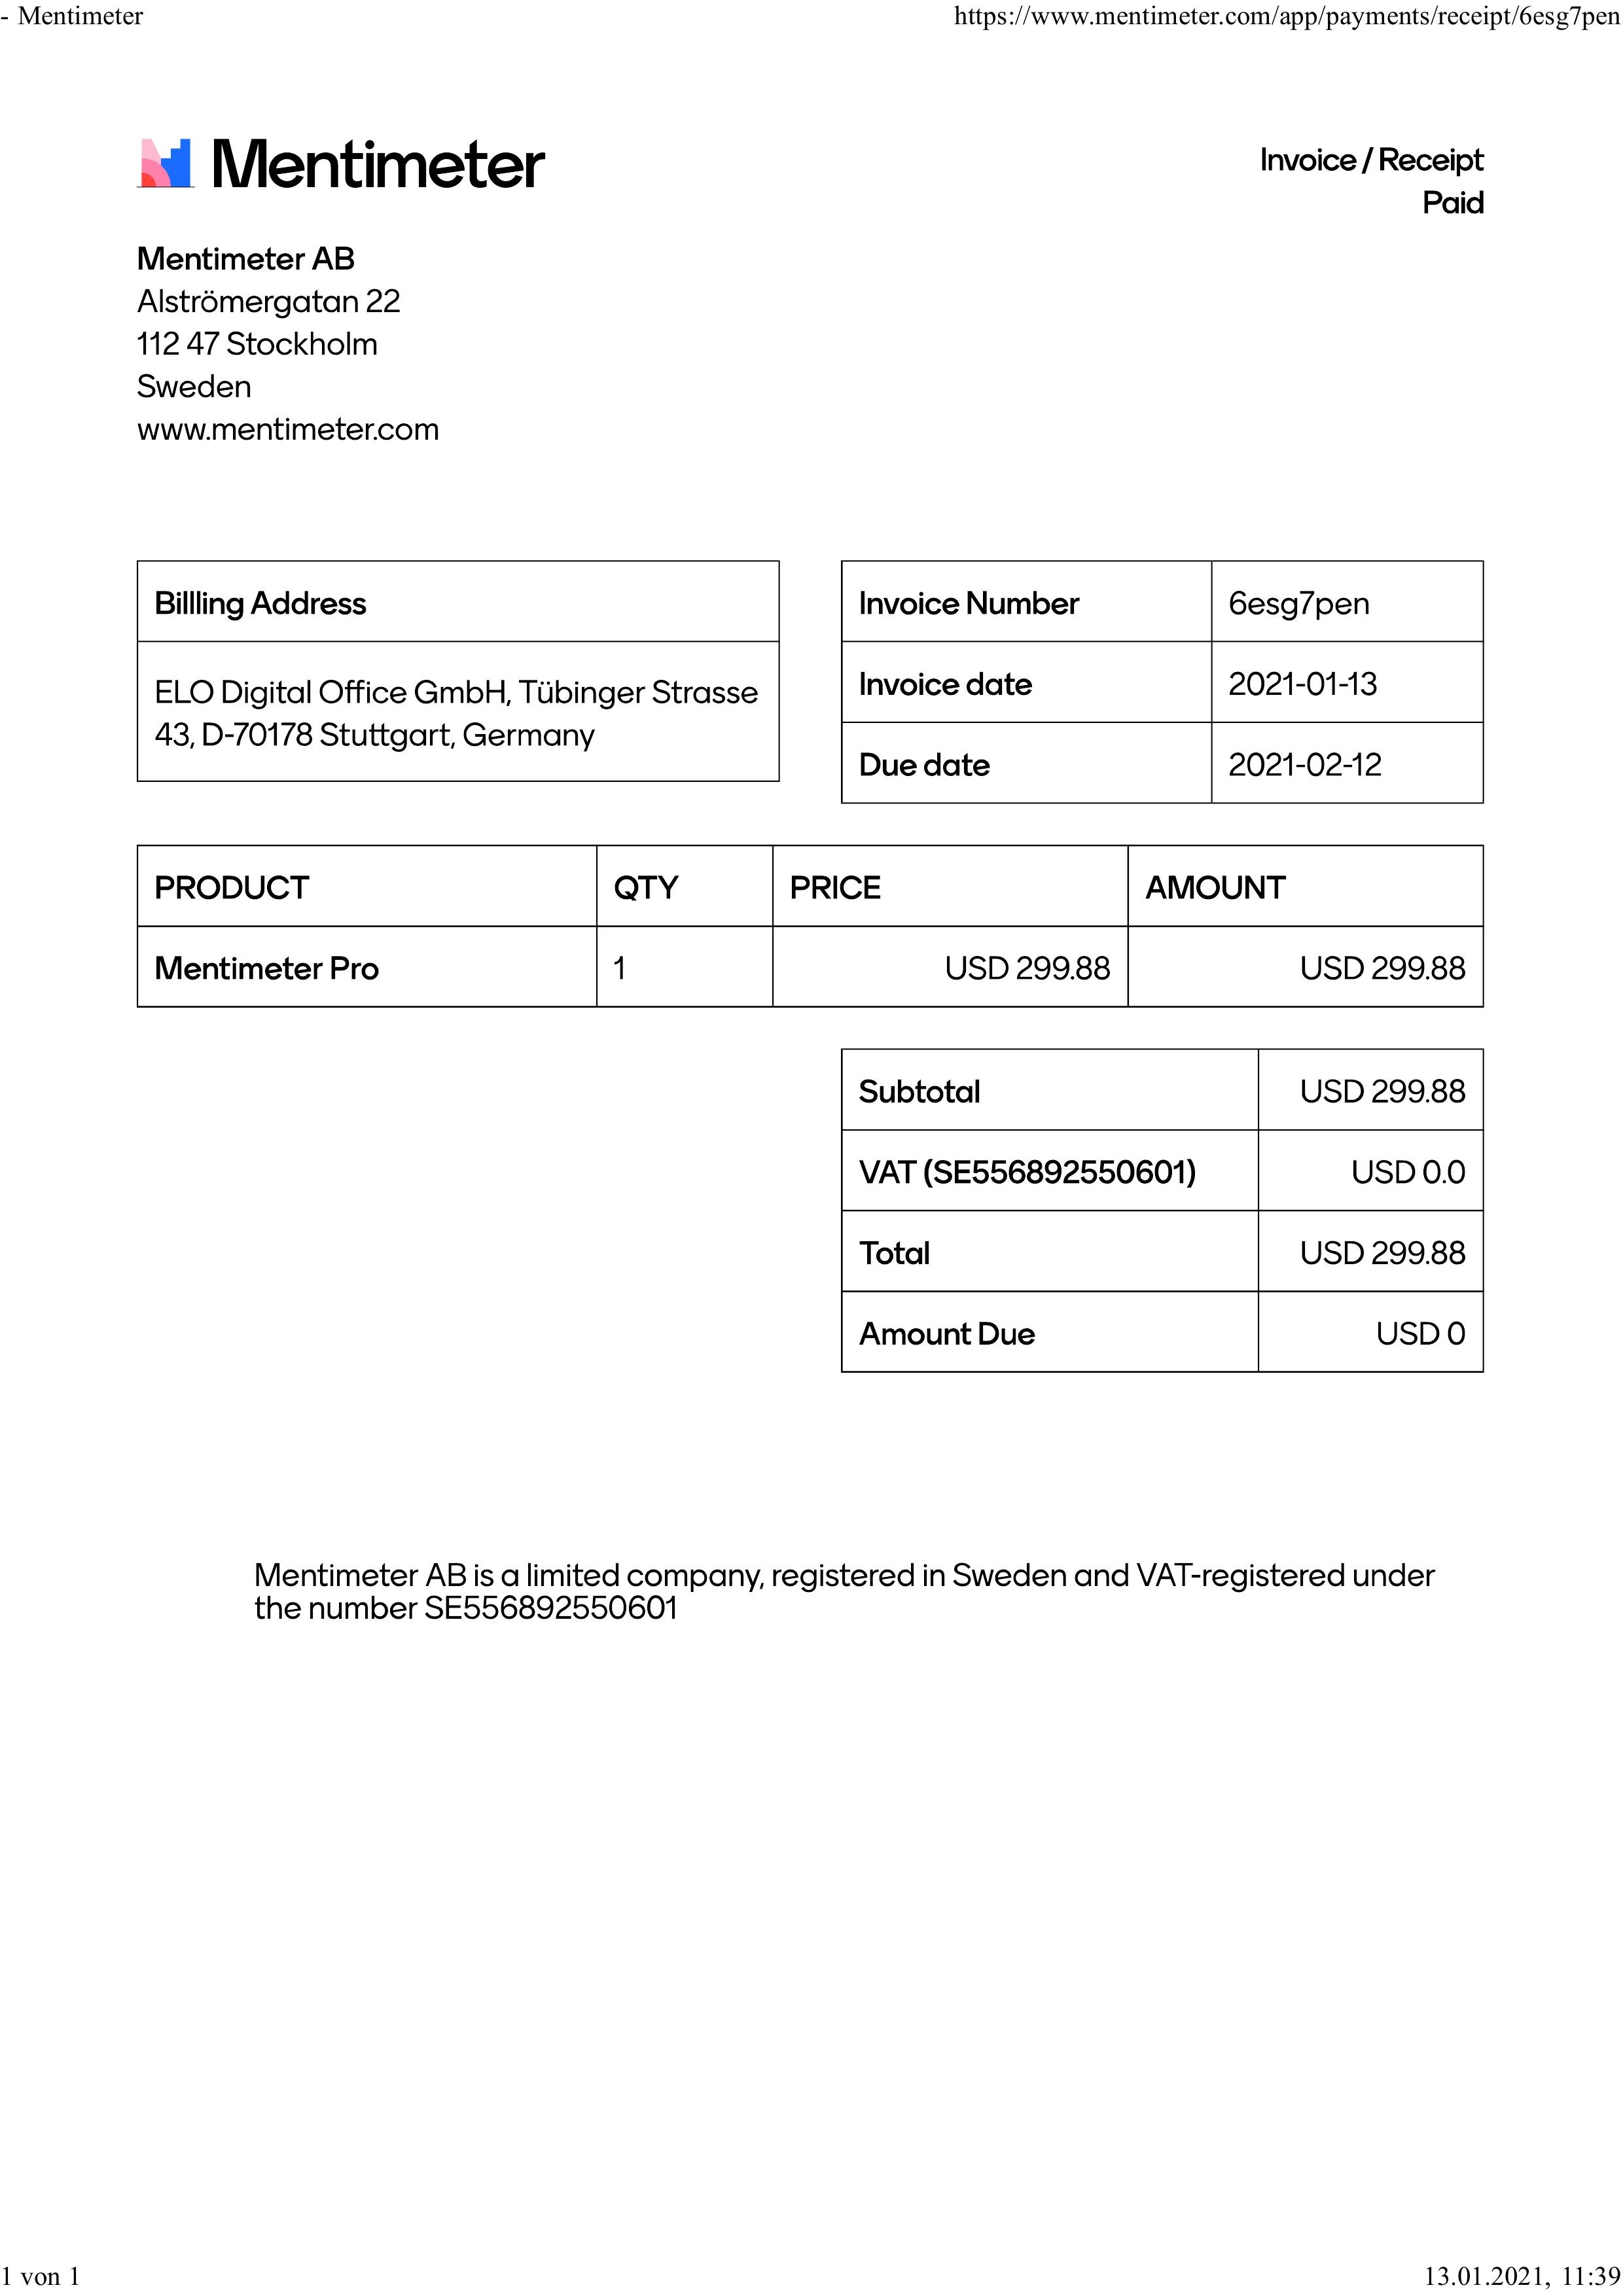
\includegraphics[width=\linewidth]{graphics/menti-invoice.jpeg} % Pfad zur Rechnungsgrafik
    \end{minipage}\hfill
    \begin{minipage}{0.45\textwidth}
        \centering
        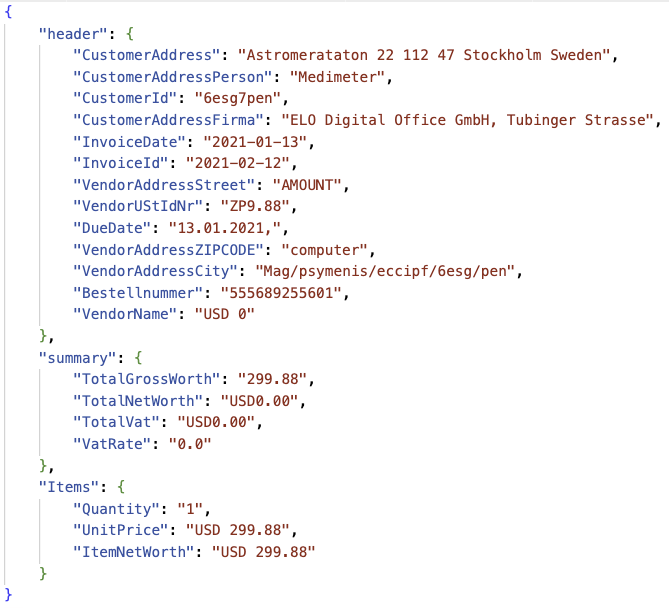
\includegraphics[width=\linewidth]{graphics/menti-json.png} % Pfad zur Donut-Inferenzgrafik
    \end{minipage}
    \caption{Gegenüberstellung von Rechnung und Inferenzergebnis von Donut}
    \label{fig:donut_inference}
\end{figure}

Unter anbetracht der in diesem Kapitel präsentierten Daten können zwei der Hypothesen verifiziert und eine falsifiziert werden:
\begin{itemize}
    \item \textbf{Hypothese 1:} Eine höhere Menge an Daten verbessert die Performance der Modelle, wobei
    eine abflachende oder sogar abfallende Wirkung bei Overfitting zu beobachten ist. Die Hypothese hat sich bestätigt. Es ist anzumerken, dass Overfitting nicht durch die Datenmenge selbst erreicht werden konnte, sondern lediglich durch Hyperparameter-Tuning. Spezifisch ist Overfitting bei allen Modellen aufgetreten, wenn die Anzahl an Epochen im Training 30 überschritten hat.
    \item \textbf{Hypothese 2:} Bei heterogenen Daten erzielt Donut bessere Ergebnisse als LayoutLMv3 und BERT. Die Hypothese ist falsifiziert. Donut hat über das Experiment hinweg schlechtere Ergebnisse erzielt als LayoutLMv3 und BERT.
    \item \textbf{Hypothese 3:} Die Qualität der vorgelagerten OCR beeinflusst die Ergebnisse von LayoutLMv3 und BERT signifikant. Die Hypothese hat sich durch die detaillierte Analyse der Inferenzergebnisse bestätigt. Die Inferenzergebnisse von LayoutLMv3 und BERT waren deutlich schlechter als die Finetuning-Ergebnisse. Dies ist auf die Verwendung von Tesseract als OCR-System zurückzuführen.
\end{itemize}

\section{Tiefere Analysen}
Die bisherigen Ergebnisse und Analysen waren sehr objektiv und bezogen sich v. a. auf die Leistungsfähigkeit der Modelle selbst. In diesen Analysen werden jedoch Faktoren außer acht gelassen, die ebenfalls eine wichtige Rolle bei der Implementierung von Modellen in Unternehmen spielen. Dieser Abschnitt betrachtet all die Faktoren, die eine signifikante Rolle spielen, bis es zu einem ersten Training kommt.

Da diese Arbeit die Anwendung von Donut im Unternehmensumfeld betrachtet, ist es wichtig, die Komplexität und Fehleranfälligkeit des Modells bei der Implementierung zu betrachten. Wie zuvor erwähnt sind die Kosten für das Training für die meisten Unternehmen nicht wirklich relevant. Die Kosten für die Rechenleistung beliefen sich bei einem Trainingsdatensatz von 850 Dokumenten, einer Schrittmenge von 100 und 30 Epochen auf 18,36 \$. Die viel größere Kostenstelle macht die Implementierung aus. Bei einem angenommenen Jahresgehalt von 55600 € pro Jahr betragen die Kosten für einen Mitarbeitenden der Entwicklung rund 29 € pro Stunde. Die Implementierung von Donut in einem Unternehmen würde jedoch nicht nur die Entwicklungskosten beinhalten. Daher ist es wichtig zu betrachten, welche Kosten bei der Implementierung von Donut in einem Unternehmen anfallen würden. Die folgend aufgeführten Erkenntnisse können nur qualitativ beschrieben werden, da eine quantitative Analyse den Rahmen dieser Arbeit sprengen würde. Die Erkenntnisse stammen aus den Erfahrungen des Entwicklungsprozesses der in Kapitel 4 beschriebenen Verarbeitungspipeline.

Die Entwicklung der Pipeline zeigte, dass Donut sehr fehleranfällig in Bezug auf seine Trainingsdaten ist. Im Annotationsprozess kann es manchmal vorkommen, dass eine JSON-Datei leere Felder enthält. Datensätze, welche mit der \textbf(datasets)-Bibliothek aufbereitet wurden, können problemlos mit leeren Feldern umgehen. Da es für das Label kein Token gibt, wird das fehlerhafte Feld in der Verarbeitung übersprungen. Wenn die Daten mit dem DonutDataset aufbereitet werden, führt bereits ein fehlerhafter Eintrag dazu, dass das gesamte Training abgebrochen wird. Dies ist ein sehr kritischer Punkt, da es sehr schwierig ist, Fehler in den Trainingsdaten zu finden. Bei kleineren Mengen ist dies noch möglich. Jedoch wird bei Mengen, die 100 Daten überschreiten, die händische Korrektur schwierig. Einen Vorteil, den das DonutDataset in diesem Zusammenhang bietet, ist dass die Daten sich bis vor die Verarbeitung vom jeweiligen Processor (s. Abb. \ref{fig:pipeline}) in einem Format von JSON und Bildern befinden. Dies ermöglicht eine für den Menschen einfache Überprüfung der Daten. Im Gegensatz dazu befinden sich die Daten bei der Verwendung der datasets-Bibliothek in einem Format, welches für den Menschen nicht ohne weiteres lesbar ist. Es ist sehr aufwendig, diese in ein lesbares Format zu bringen. Das Zurückführen von Fehlern auf bestimmte Daten sehr schwierig. Jedoch kam es nie zu einem Abbruch des Trainingsprozesses bei LayoutLMv3 oder BERT. Jedoch kam es sehr häufig zu einem Abbruch beim Training von Donut. Dies ist ein entscheidender Schwachpunkt, der bei der Implementierung von Donut in einem Unternehmen berücksichtigt werden sollte.

Die Trainingszeiten sind ebenfalls ein wichtiger Faktor in der Kostenrechnung. Abseits der bereits präsentierten GPUh soll eine kurze Betrachtung erfolgen, wie sich die Trainingszeiten zusammensetzen. Bei Donut ist aufgefallen, dass über 40 \% der Trainingszeit auf die Validierung entfallen. Während es bei LayoutLMv3 und BERT für 80 Validierungsdaten nur wenige Sekunden dauert, bis die Validierung in einer Epoche abgeschlossen ist, dauert es bei Donut mehrere Minuten. Wie dieser Zeitunterschied zustande kommt, konnte nicht weiter untersucht werden. Es wurden mehrere Argumentationen basierend auf der Architektur von Donut vorgeschlagen. Keine Erklärung kann jedoch als gesichert angesehen werden. Daher überlässt es diese Bachelorarbeit künftigen Arbeiten eine Erklärung für diesen Sachverhalt zu finden. Dies hat nicht nur zur Folge, dass die benötigten GPUh steigen, sondern auch, dass beim Testen des Finetunings mehr Zeit benötigt wird. 

Zuletzt gilt es zu betrachten, wie Modelle auf unterschiedliche Hyperparameter reagieren. Die initiale Hyperparameterkonfiguration sieht wie folgt aus:
\begin{itemize}
    \item \textbf{Learning Rate:} 3e-5 - Bestimmt, wie schnell oder langsam das Modell während des Trainings lernt.
    \item \textbf{Per-device Train Batch Size:} 2 - Bestimmt, wie viele Datenpunkte das Modell auf einmal verarbeitet.
    \item \textbf{Per-device Eval Batch Size:} 2
    \item \textbf{Epochs:} 30 - Bestimmt, wie oft das Modell über den gesamten Datensatz trainiert wird.
    \item \textbf{Val-check-interval:} 0.1 - Bestimmt, wie häufig das Modell während einer Epoche validiert wird (in diesem Fall 40 \% der Trainingsschritte pro Epoche)
    \item \textbf{Check-val-every-n-epoch:} 3 - Das Modell wird alle drei Epochen auf Validierungsdaten überprüft. 
    \item \textbf{Warmup Steps:} 81 - Anzahl der Schritte zu Beginn des Trainings, in denen die Lernrate schrittweise erhöht wird. 
\end{itemize}
Die Hyperparameterkonfiguration wurde für alle Modelle gleich gewählt. Es ist jedoch zu erwähnen, dass die Hyperparameterkonfiguration für jedes Modell individuell optimiert werden sollte. Die Hyperparameterkonfiguration hat einen signifikanten Einfluss auf die Modellperformance und die Trainingszeit. Die Analyse der Trainings ergab, dass die Hyperparameterkonfiguration für das Training aller Modelle nicht optimal ist. Zunächst wird in Abb. \ref{fig:flattening} deutlich, dass ab einer gewissen Anzahl an Trainingsschritten die Änderungsrate von F1-Score abflacht. In diesem Beispiel schwankte der F1-Score mit 0.5 \% um den Wert von 93.6 \%. Die folgenden Trainingsschritte schwanken anschließend um einen bestimmten Wert. Nachdem dieser Schritt erreicht ist, wird das Modell unnötig weitertrainiert, da keine Verbesserung mehr stattfindet. Eine Senkung der Epochen auf 20 konnte hier für alle Modelle ein Drittel der Trainingszeit einsparen. Die Validierung pro Epoche konnte auf 40 \% reduziert werden. Es entstand kein nennenswerter Verlust von F1. Die Lernrate war mit 3e-5 für alle Modelle zu niedrig. Eine Erhöhung auf 1e-5 konnte in viel kürzerer Zeit die zuvor präsentierten Ergebnisse erreichen. Die Instabilität stieg nicht nennenswert an. Eine Erhöhung der Batch Size hatte keinen nennenswerten Effekt auf die Trainingszeit. Schlussendlich führte eine Reduktion der Anzahl an Validierungen zu einer Verschlechterung des F1-Scores von bis zu 7 \% bei Donut und einer Verschlechterung der Accuracy von rund 5 \%. Eine Erhöhung der Validierungen führte zu keiner Verbesserung der Metriken, jedoch stieg die Trainingszeit v. a. für Donut unter Anbetracht der verlängerten Validierungszeit erheblich. Unter Beachtung dieser Ergebnisse wurde für das Erreichen der besten Ergebnisse (s. Tab \ref{tab:best_results}) folgende Konfiguration verwendet:
\begin{itemize}
    \item \textbf{Learning Rate:} 3e-5
    \item \textbf{Per-device Train Batch Size:} 2
    \item \textbf{Per-device Eval Batch Size:} 2
    \item \textbf{Epochs:} 20
    \item \textbf{Val-check-interval:} 0.4
    \item \textbf{Check-val-every-n-epoch:} 3
    \item \textbf{Warmup Steps:} 81
\end{itemize}

\section{Zusammenfassende Bewertung}
In Kapitel 5 wurden die Ergebnisse der empirischen Untersuchung präsentiert, die die Leistungsfähigkeit des Donut-Modells im Vergleich zu den etablierten OCR-basierten Modellen LayoutLMv3 und BERT unter realen Anwendungsbedingungen evaluiert haben. Dabei standen die Metriken Accuracy, F1-Score und GPU-Stunden im Fokus, um ein umfassendes Bild der Modellperformance zu liefern.

Die Analyse der Ergebnisse zeigt, dass Donut in allen drei betrachteten Metriken hinter seinen Konkurrenten zurückbleibt. Insbesondere bei der Accuracy und dem F1-Score erreicht Donut niedrigere Werte, was auf eine geringere Fähigkeit hinweist, relevante Informationen korrekt zu extrahieren und falsch positive Ergebnisse zu minimieren. Obwohl die GPU-Stunden anzeigen, dass Donut eine höhere Rechenzeit benötigt, liegen die absoluten Kosten für die Rechenleistung in einem sehr geringen Bereich, was die finanziellen Implikationen relativiert.

Für die praktische Anwendung bedeutet dies, dass Donut, obwohl es in der Lage ist, eine automatisierte Dokumentenverarbeitung zu unterstützen, möglicherweise nicht die optimale Wahl für Anwendungsfälle ist, die eine hohe Genauigkeit erfordern. Dies gilt insbesondere in Umgebungen, in denen die Verfügbarkeit von Trainingsdaten begrenzt ist, da Donut eine größere Datenmenge zur Optimierung seiner Leistung benötigt. Die Ergebnisse deuten darauf hin, dass Donut besonders in homogenen Anwendungsszenarien mit ausreichenden Trainingsdaten und weniger kritischen Genauigkeitsanforderungen eine kosteneffiziente Lösung sein könnte.

Die höhere Ressourcenanforderung und die längeren Trainingszeiten, besonders im Hinblick auf die Validierung, sind weitere Aspekte, die bei der Implementierung von Donut in Betracht gezogen werden sollten. Es ist daher empfehlenswert, die Einsatzmöglichkeiten von Donut genau zu prüfen und gegen die potenziellen operativen Einschränkungen abzuwägen.

Die kritische Bewertung der Modelle zeigt, dass LayoutLMv3 und BERT, obwohl sie abhängig von der Qualität der vorgeschalteten OCR sind, eine robustere und effizientere Leistung in Bezug auf die Dokumentenverarbeitung bieten. Dies unterstreicht die Bedeutung der Wahl des richtigen Tools für spezifische Anwendungsbedingungen und Zielsetzungen. Es wird deutlich, dass die Entscheidung für ein Modell nicht nur auf der Basis der reinen Performance getroffen werden sollte, sondern auch operationale und ökonomische Überlegungen einbeziehen muss.

Zusätzlich zur Evaluation der Modellperformance wurden auch spezifische Hypothesen bezüglich der Auswirkungen der Datensatzgröße und der Modellwahl bei heterogenen Daten untersucht. Die erste Hypothese, dass eine höhere Menge an Daten die Modellperformance verbessert, konnte bestätigt werden, obwohl eine abflachende Wirkung bei zunehmender Datensatzgröße beobachtet wurde. Die zweite Hypothese, dass Donut bei heterogenen Daten bessere Ergebnisse als LayoutLMv3 und BERT erzielt, musste jedoch verworfen werden. Donut zeigte durchgehend schwächere Leistungen als die Vergleichsmodelle, was darauf hinweist, dass es trotz seiner spezialisierten Architektur möglicherweise nicht die beste Wahl für extrem heterogene Daten ist. Ferner wurde bestätigt, dass die vorgelagerte OCR-Engine vor den OCR-abhängigen Modellen einen großen Einfluss auf die Modellperformance hat.

Zusammenfassend lassen sich die Schlüsselergebnisse dahingehend interpretieren, dass Donut in der Lage ist, eine Unterstützungsfunktion in der Dokumentenverarbeitung zu übernehmen, jedoch Limitationen aufweist, die bei der praktischen Implementierung berücksichtigt werden müssen. Diese Erkenntnisse bieten eine wichtige Grundlage für die folgenden Kapitel, in denen die Implikationen für die Praxis weiter vertieft und diskutiert werden.
\chapter{Diskussion und kritische Betrachtung der Forschung}
In diesem Kapitel werden die in Kapitel 5 präsentierten Ergebnisse eingehend diskutiert, um tiefere Einblicke in die Implikationen der Forschungsergebnisse für praktische Anwendungen zu gewinnen. Dabei wird zunächst auf die Auswirkungen der Modellperformance auf Geschäftsprozesse und die potenziellen Anwendungsbereiche der untersuchten Modelle eingegangen. Dies umfasst sowohl die direkten Auswirkungen der Nutzung von Document Understanding Transformers in realen Unternehmenskontexten als auch die strategischen Überlegungen, die Unternehmen anstellen sollten, wenn sie erwägen, solche Technologien zu implementieren.

Des Weiteren werden die Limitationen der durchgeführten Studie kritisch reflektiert. Es wird diskutiert, inwiefern die gewählten Methoden, die Datensätze und die experimentellen Bedingungen möglicherweise zu Verzerrungen in den Ergebnissen geführt haben könnten. Diese Diskussion ist entscheidend, um die Validität und Reliabilität der Studienergebnisse zu verstehen und ihre Generalisierbarkeit einschätzen zu können.

Abschließend wird ein Ausblick für zukünftige Forschungsarbeiten gegeben. Es werden Empfehlungen ausgesprochen, welche Aspekte in folgenden Studien berücksichtigt werden sollten, um die Forschung im Bereich der automatisierten Dokumentenverarbeitung voranzutreiben. Diese Empfehlungen basieren auf den erkannten Forschungslücken und den während der Studie gewonnenen Erkenntnissen. Dabei wird insbesondere auf die Notwendigkeit eingegangen, weitere innovative Ansätze zu entwickeln, die die Limitationen bestehender Modelle überwinden können.

\section{Implikationen für die Praxis}
Wie bereits in Kapitel 5 erwähnt, erzielt Donut gute Ergebnisse, die aber nicht mit den Ergebnissen von OCR-basierten Modellen mithalten können. Von daher ist es fraglich, ob der Einsatz von Document Understanding Transformer Modellen in der vollständigen Automatisierung sinnvoll ist. Jedoch bietet der Donut Ansatz einige Vorteile, die in der Praxis genutzt werden können. Wie bereits erwähnt, kann Donut die manuelle Dokumentenverarbeitung deutlich effizienter gestalten, indem es eine große Anzahl von Entitäten in Dokumenten bereits im Vorhinein erkennt und lediglich c.a. 20 \% der Entitäten manuell überprüft werden müssen. Dies kann die Bearbeitungszeit von Dokumenten erheblich reduzieren und somit die Effizienz der Dokumentenverarbeitung steigern. Ein weiterer Vorteil ist, dass sowohl das Training als auch die Inferenz von Donut sehr schnell und kostengünstig sind. Unternehmen, welche die interne automatisiert Dokumentenverarbeitung einführen möchten, können von diesen Vorteilen profitieren. In der Endanwendung ELO enterprise wird bspw. eine serverseitige Extraktionskomponente verwendet, die zwar sehr genau ist, aber auch sehr teuer und rechenintensiv. Donut könnte hier eine kostengünstige und effiziente Alternative darstellen. Wenn der Anspruch an die Genauigkeit nicht so hoch ist, kann Donut eine gute Lösung sein. Des Weiteren hat Donut den Vorteil, dass das Model auf der Clientseite ausgeführt wird und somit keine Daten an Dritte weitergegeben werden. Dies kann für Unternehmen, die großen Wert auf Datenschutz legen, ein entscheidender Faktor sein. In der Inferenz ist Donut auch nicht von GPUs abhängig, sondern kann auf CPUs in kurzer Zeit Daten verarbeiten. 

In diesem Zusammenhang ist anzumerken, dass die Donut-Pipeline so aufbereitet wurde, dass sie mit wenig Anpassungsaufwand in die Endanwendung integriert werden kann. Dies ist nicht Teil dieser Arbeit, da zu diesem Zeitpunkt noch nicht feststeht, ob Donut in der Endanwendung ELO enterprise integriert wird. Im Falle der Implementierung liefert Donut in der Inferenz die extrahierten Entitäten an die Endanwendung als JSON, welche diese dann weiterverarbeiten kann. Die Donut-Komponente kann in diesem Fall auch auf der Clientseite ausgeführt werden und benötigt keine zusätzlichen Ressourcen auf dem Server oder eine entsprechende Schnittstelle.

Ein weiterer wichtiger Punkt in der Praxis sind die Trainingsdaten und ihre Verfügbarkeit. Die meisten Unternehmen werden nicht über ausreichend annotierte Trainingsdaten verfügen, um ein Modell wie Donut zu trainieren. In diesem Fall kann auf Transfer Learning zurückgegriffen werden. Donut kann auf einem allgemeinen Datensatz wie FUNSD oder CORD vortrainiert werden und anschließend auf den Unternehmensdaten feinabgestimmt werden. Dies kann die Anforderungen an die Trainingsdaten erheblich reduzieren und den Implementierungsaufwand verringern. Dieser Ansatz wurde auch in dieser Arbeit gewählt. Allerdings kann es für Unternehmen schwierig sein, selbst einen kleinen Datensatz für das Finetuning zu annotieren. In diesem Fall kann auf externe Anbieter zurückgegriffen werden, die die Annotationen durchführen. Hier muss eine Abwägung zwischen Kosten der Annotation von externen Anbietern und der händischen Annotation durch Mitarbeiter getroffen werden. Des weiteren muss definiert werden, wie hoch der Anspruch an die Genauigkeit der Annotationen ist. Externe Annotationstools wie das Azure Document Intelligence Studio können zwar günstiger sein, liefern aber auch oft ungenauere Annotationen.

Die Diskussion über Trainingsdaten aus kommerzieller Sicht ist besonders relevant, da die Qualität und Verfügbarkeit von annotierten Daten oft die größte Hürde für die Implementierung fortgeschrittener maschineller Lernmodelle in Unternehmen darstellt. Die Anschaffung qualitativ hochwertiger, spezifisch annotierter Daten kann sehr kostspielig sein, insbesondere wenn es um seltene oder spezielle Dokumententypen geht, die für bestimmte Geschäftsanwendungen erforderlich sind. Unternehmen müssen daher die Kosten für die Datensammlung und -annotation gegen den erwarteten Nutzen abwägen.

Ein wichtiger Aspekt ist, dass die Investition in qualitativ hochwertige Trainingsdaten eine langfristige Investition in die Automatisierung und Effizienzsteigerung darstellen kann. Hochwertige Daten verbessern nicht nur die Leistung der Modelle, sondern verringern auch das Risiko von Fehlinterpretationen und Fehlern in der automatisierten Verarbeitung, was wiederum die Notwendigkeit manueller Eingriffe reduziert und die Gesamtzuverlässigkeit der Systeme erhöht. Unternehmen, die in der Lage sind, in diese Anfangsinvestitionen zu investieren, könnten eine schnellere Amortisierung und höhere Renditen in Form von Effizienzsteigerungen sehen.

Zusätzlich zur Eigenproduktion von Trainingsdaten kann die Nutzung von syntaktisch generierten oder semi-synthetischen Daten eine kosteneffiziente Alternative bieten. Durch Techniken wie Data Augmentation können bestehende Datensätze erweitert werden, um die Robustheit und Generalisierungsfähigkeit der Modelle zu verbessern, ohne die Kosten für die manuelle Annotation neuer Daten tragen zu müssen. Dies kann besonders nützlich sein, um Modelle gegenüber speziellen Szenarien zu stärken, die in den ursprünglichen Trainingsdaten unterrepräsentiert sind.

%%% Ende des eigentlichen Inhalts %%%

% chapter  (end)

%%% Quellenverzeichnisse (keine Anpassung nötig) %%%
\clearpage
\literaturverzeichnis
%%% Ende Quellenverzeichnisse %%%

\clearpage
\clearpage

\thispagestyle{empty}

{\LARGE\textsf{\textbf{Erklärung zur Verwendung generativer KI-Systeme}}\bigskip}

Bei der Erstellung der eingereichten Arbeit habe ich die nachfolgend aufgeführten auf künstlicher Intelligenz (KI) basierten Systeme benutzt:
% HIER EDITIEREN: (Immer mit \item einen neuen Antrag anführen
\begin{enumerate}
  \item
\end{enumerate}

Ich erkläre, dass ich
\begin{itemize}
  \item mich aktiv über die Leistungsfähigkeit und Beschränkungen der oben genannten KI-Systeme informiert habe, \footnote{U. a. gilt es hierbei zu beachten, dass an KI weitergegebene Inhalte ggf. als Trainingsdaten genutzt und wiederverwendet werden. Dies ist insb. für betriebliche Aspekte als kritisch einzustufen.}
  \item die aus den oben angegebenen KI-Systemen direkt oder sinngemäß übernommenen Passagen gekennzeichnet habe, \footnote{In der Fußnote Ihrer Arbeit geben Sie die KI als Quelle an, z.B.: Erzeugt durch Microsoft Copilot am dd.mm.yyyy. Oder: Entnommen aus einem Dialog mit Perplexity vom dd.mm.yyyy. Oder Absatz 2.3 wurde durch ChatGPT sprachlich geglättet.}
  \item überprüft habe, dass die mithilfe der oben genannten KI-Systeme generierten und von mir übernommenen Inhalte faktisch richtig sind, \footnote{Beispiele hierfür sind u.a. die folgenden Arbeitsschritte: Generierung von Ideen, Konzeption der Arbeit, Literatursuche, Literaturanalyse, Literaturverwaltung, Auswahl von Methoden, Datensammlung, Datenanalyse, Generierung von Programmcodes.}
  \item mir bewusst bin, dass ich als Autorin bzw. Autor dieser Arbeit die Verantwortung für die in ihr gemachten Angaben und Aussagen trage.
\end{itemize}

\vspace{1cm}

Die oben genannten KI-Systeme habe ich wie im Folgenden dargestellt eingesetzt:
\begin{center}
  \begin{tabular}{| p{0.25\linewidth} | p{0.2\linewidth} | p{0.5\linewidth} |}
    \hline
    \textbf{Arbeitsschritt in der wissenschaftlichen Arbeit} & \textbf{Eingesetzte(s) KI-System(e)} & \textbf{Beschreibung der Verwendungsweise} \\
    \hline
    % HIER EDITIEREN: (Nächste Zeile beliebig oft kopieren)
                                                             &                                      &                                            \\
    \hline
  \end{tabular}
\end{center}



%%% Erklärung (keine Anpassungen nötig) %%%
% steht ganz am Ende des Dokuments
\cleardoublepage
\clearpage

\thispagestyle{empty}

{\LARGE\textsf{\textbf{Erklärung}}\bigskip}

% \typMeinerArbeit und \themaMeinerArbeit werden in deckblatt.tex definiert
Ich versichere hiermit, dass ich die vorliegende Arbeit mit dem Thema: \emph{\themaMeinerArbeit} selbstständig verfasst und keine anderen als die angegebenen Quellen und Hilfsmittel benutzt habe.
Ich versichere zudem, dass die eingereichte elektronische Fassung mit der gedruckten Fassung übereinstimmt.

\vspace{3cm}

\begin{center}
  \begin{tabular}{ccc}
    (Ort, Datum) & \hspace{0.3\linewidth} & (Unterschrift)
  \end{tabular}
\end{center}
\end{document}
